\documentclass[11pt]{article}
\usepackage[utf8]{inputenc}
\usepackage[pdftex]{graphicx}
\usepackage{pdfpages}
\usepackage[english]{babel}
\usepackage [autostyle, english = american]{csquotes}
\usepackage{mathtools}
\usepackage{float}
\usepackage{xcolor}
\usepackage{listings}
\usepackage{fancyvrb}
\usepackage{caption,subcaption}
%\usepackage{subfigure}
\usepackage[margin=0.6in]{geometry}
\usepackage[export]{adjustbox}
\usepackage{listings}
\usepackage{hyperref}
\usepackage{wrapfig}
\usepackage{newfloat}
\usepackage[cm]{fullpage}
\usepackage[cachedir=build,newfloat,outputdir=build]{minted}
\usepackage{verbatim}
\usepackage{tikz}
\usetikzlibrary{decorations.pathmorphing,positioning}

\tikzset{mydeco/.style={decoration={random steps,segment length=.08em,amplitude=.05em},decorate,line cap=round}}

\tikzset{anarchy/.pic={
    \draw[line width=.1em,mydeco,decorate,red,fill=red](0em,0em)--(1.2em,.3em)--cycle;
    \draw[line width=.1em,mydeco,red,fill=red](.2em,-.3em)--(.5em,.7em)--cycle;
    \draw[line width=.1em,mydeco,red,fill=red](.5em,.7em)--(.8em,-.3em)--cycle;
    \draw[line width=.1em,red,line cap=round,mydeco](.5em,.2em) circle(.6em);
}}

\newcommand{\anarchy}{\tikz\pic{anarchy};}

\definecolor{mintedbackground}{rgb}{0,0,0}
\usemintedstyle{tango}
\newenvironment{code}{\captionsetup{type=listing}}{}
\SetupFloatingEnvironment{listing}{name=Source Code}
\captionsetup[subfigure]{subrefformat=simple,labelformat=simple}
\renewcommand{\thelisting}{\arabic{listing}}
\renewcommand\thesubfigure{(\alpha{subfigure})}
\definecolor{lightgray}{rgb}{.7,.7,.7}
\definecolor{gray}{rgb}{.4,.4,.4}
\definecolor{darkblue}{rgb}{0,0,.3}
\definecolor{gray}{rgb}{0.4,0.4,0.4}
\definecolor{darkblue}{rgb}{0.0,0.0,0.6}
\definecolor{cyan}{rgb}{0.0,0.6,0.6}
\renewcommand{\thelisting}{\arabic{listing}}
\renewcommand\thesubfigure{(\alph{subfigure})}

\definecolor{termback}{HTML}{DBE0E0}
\definecolor{termkeyword}{HTML}{50DA8B}
\lstdefinestyle{Bash}
{language=bash,
keywordstyle=\color{termkeyword},
basicstyle=\ttfamily,
morekeywords={@.},
alsoletter={:~\$.},
morekeywords=[2]{peter@kbpet:},
keywordstyle=[2]{\color{termkeyword}},
literate={\$}{{\textcolor{termkeyword}{\$}}}1 
         {:}{{\textcolor{termkeyword}{:}}}1
         {~}{{\textcolor{termkeyword}{\textasciitilde}}}1,
}

\geometry{
 a4paper,
 total={170mm,257mm},
 left=10mm,
 right=10mm,
 top=10mm,
 bottom=15mm
}
\graphicspath{ {images/} }

\lstset{
  basicstyle=\ttfamily,
  columns=fullflexible,
  showstringspaces=false,
  commentstyle=\color{gray}\upshape
}

\hypersetup{
    colorlinks,
    citecolor=black,
    filecolor=black,
    linkcolor=black,
    urlcolor=blue
}
 \newmintedfile[pycode]{python3}{
frame=lines,
framesep=2mm,
fontsize=\footnotesize,
showtabs =false,
autogobble=true,
breaklines=true,
mathescape=true
}
 \newmintedfile[shellcode]{bash}{
frame=lines,
framesep=2mm,
fontsize=\footnotesize,
showtabs =false,
autogobble=true,
breaklines=true,
mathescape=true
}

\newmintedfile[rcode]{S}{
frame=lines,
framesep=2mm,
fontsize=\footnotesize,
showtabs =false,
autogobble=true,
breaklines=true,
mathescape=true
}
\newmintinline[ibash]{bash} {
}

\newmintinline[ipy]{python3} {
}

\newmintinline[ir]{S} {
}
\RecustomVerbatimCommand{\VerbatimInput}{VerbatimInput}%
{fontsize=\footnotesize,
 %
 frame=lines,  % top and bottom rule only
 framesep=2em, % separation between frame and text
 %
 labelposition=topline,
 %
 commandchars=\|\(\), % escape character and argument delimiters for
                      % commands within the verbatim
 commentchar=*        % comment character
}

\newcommand*{\escape}[1]{\texttt{\textbackslash#1}}
\newcommand{\dfa}[3]{\ir{#1#2#3}}

\newcommand{\rpm}{\sbox0{$1$}\sbox2{$\scriptstyle\pm$}
  \raise\dimexpr(\ht0-\ht2)/2\relax\box2 }

\title{Assignment 5 \\ Introduction to Information Retrieval \\ CS734/834}
\author{John Berlin}
\date{\today}
\renewcommand\thesection{Q.\arabic{section}}
\renewcommand\thesubsection{\thesection}
\begin{document}
\maketitle
\newpage
\section*{Note}
In order to making the computation of the iterations for Hits and Pagerank stop at the desired iteration for \autoref{q1}, I modified the respective algorithm implementations that the NetworkX\footnote{\href{http://networkx.readthedocs.io/en/networkx-1.10/}{http://networkx.readthedocs.io/en/networkx-1.10/}} library provides. The modifications were only done so that they do not throw an exception if convergence was not reached when the stopping point parameter \textit{max\_iter} was hit.  These changes can be seen in \autoref{code:nxc}. Also utilized in \autoref{q1} are three new context classes were created GraphBuilder,AutoSLatexTable, and AutoSaveTwoFileTypes. GraphBuilder creates a new networkx Graph and populates it from the given configuration. 
AutoSLatexTable is similar to the other autosaver classes discussed in this section for Q4 but it creates a latex table utilizing the tabulate library\footnote{\href{https://pypi.python.org/pypi/tabulate}{https://pypi.python.org/pypi/tabulate}}. AutoSaveTwoFileTypes allows usage of two autosavers from a given configuration containing the required arguments for each.
\newpage
\section{Question 10.3} \label{q1}
\begin{verbatim}
Compute five iterations of HITS (see Algorithm 3) and PageRank (see Fig-
ure 4.11) on the graph in Figure 10.3. Discuss how the PageRank scores compare
to the hub and authority scores produced by HITS
\end{verbatim}
\subsection*{Answer} 
The networkx library was utilized to answer this question and node,edges files used when creating the graphs can be found in the data folder that companies this report. After computing each iteration the respective iterations scores were save to files for use by \autoref{code:q1r} to generate the respective iterations graph plot, the python code for this question can be seen in \autoref{code:q1p}. Please note that the score label for node seven in  \autoref{fig:q1_i1} through \autoref{fig:q1_i5} has a pagerank of 0.7 throughout. This happens due to the cutting short of the algorithms iterations which was necessary to answer this question.  

After the first iteration \autoref{fig:q1_i1} the scores for each node begin to show who are the good hubs or authorities. Node one and six have interesting values from the hits algorithm. Both nodes authority scores are the highest out of the others likewise with the pagerank score. The other nodes scores show that they are more hubs than authorities except node five which has all three scores present. Iterations two \autoref{fig:q1_i2} through five  \autoref{fig:q1_i5} show that only nodes five and one have value changes and all other node values stay the same. This leads me to believe that due to the limited size of this graph that it only took two iterations to determine the final graph. When only considering pagerank scores it would be hard to determine who was an authority, a hub or both. 

This can be seen in nodes five,three,two and four. Node five who is both an authority and a hub has a pagerank score of 0.11 whereas nodes three, two and four have pagerank scores of 0.07 but node three has a hub score of 0.45 unlike the others who with 0.2. These nodes pagerank score difference from node 5 is only 0.04 which is small enough that without prior knowledge of the graph using pagerank as an indicator for who was a hub or an authority would be hard.
\begin{figure}[H]
\centering
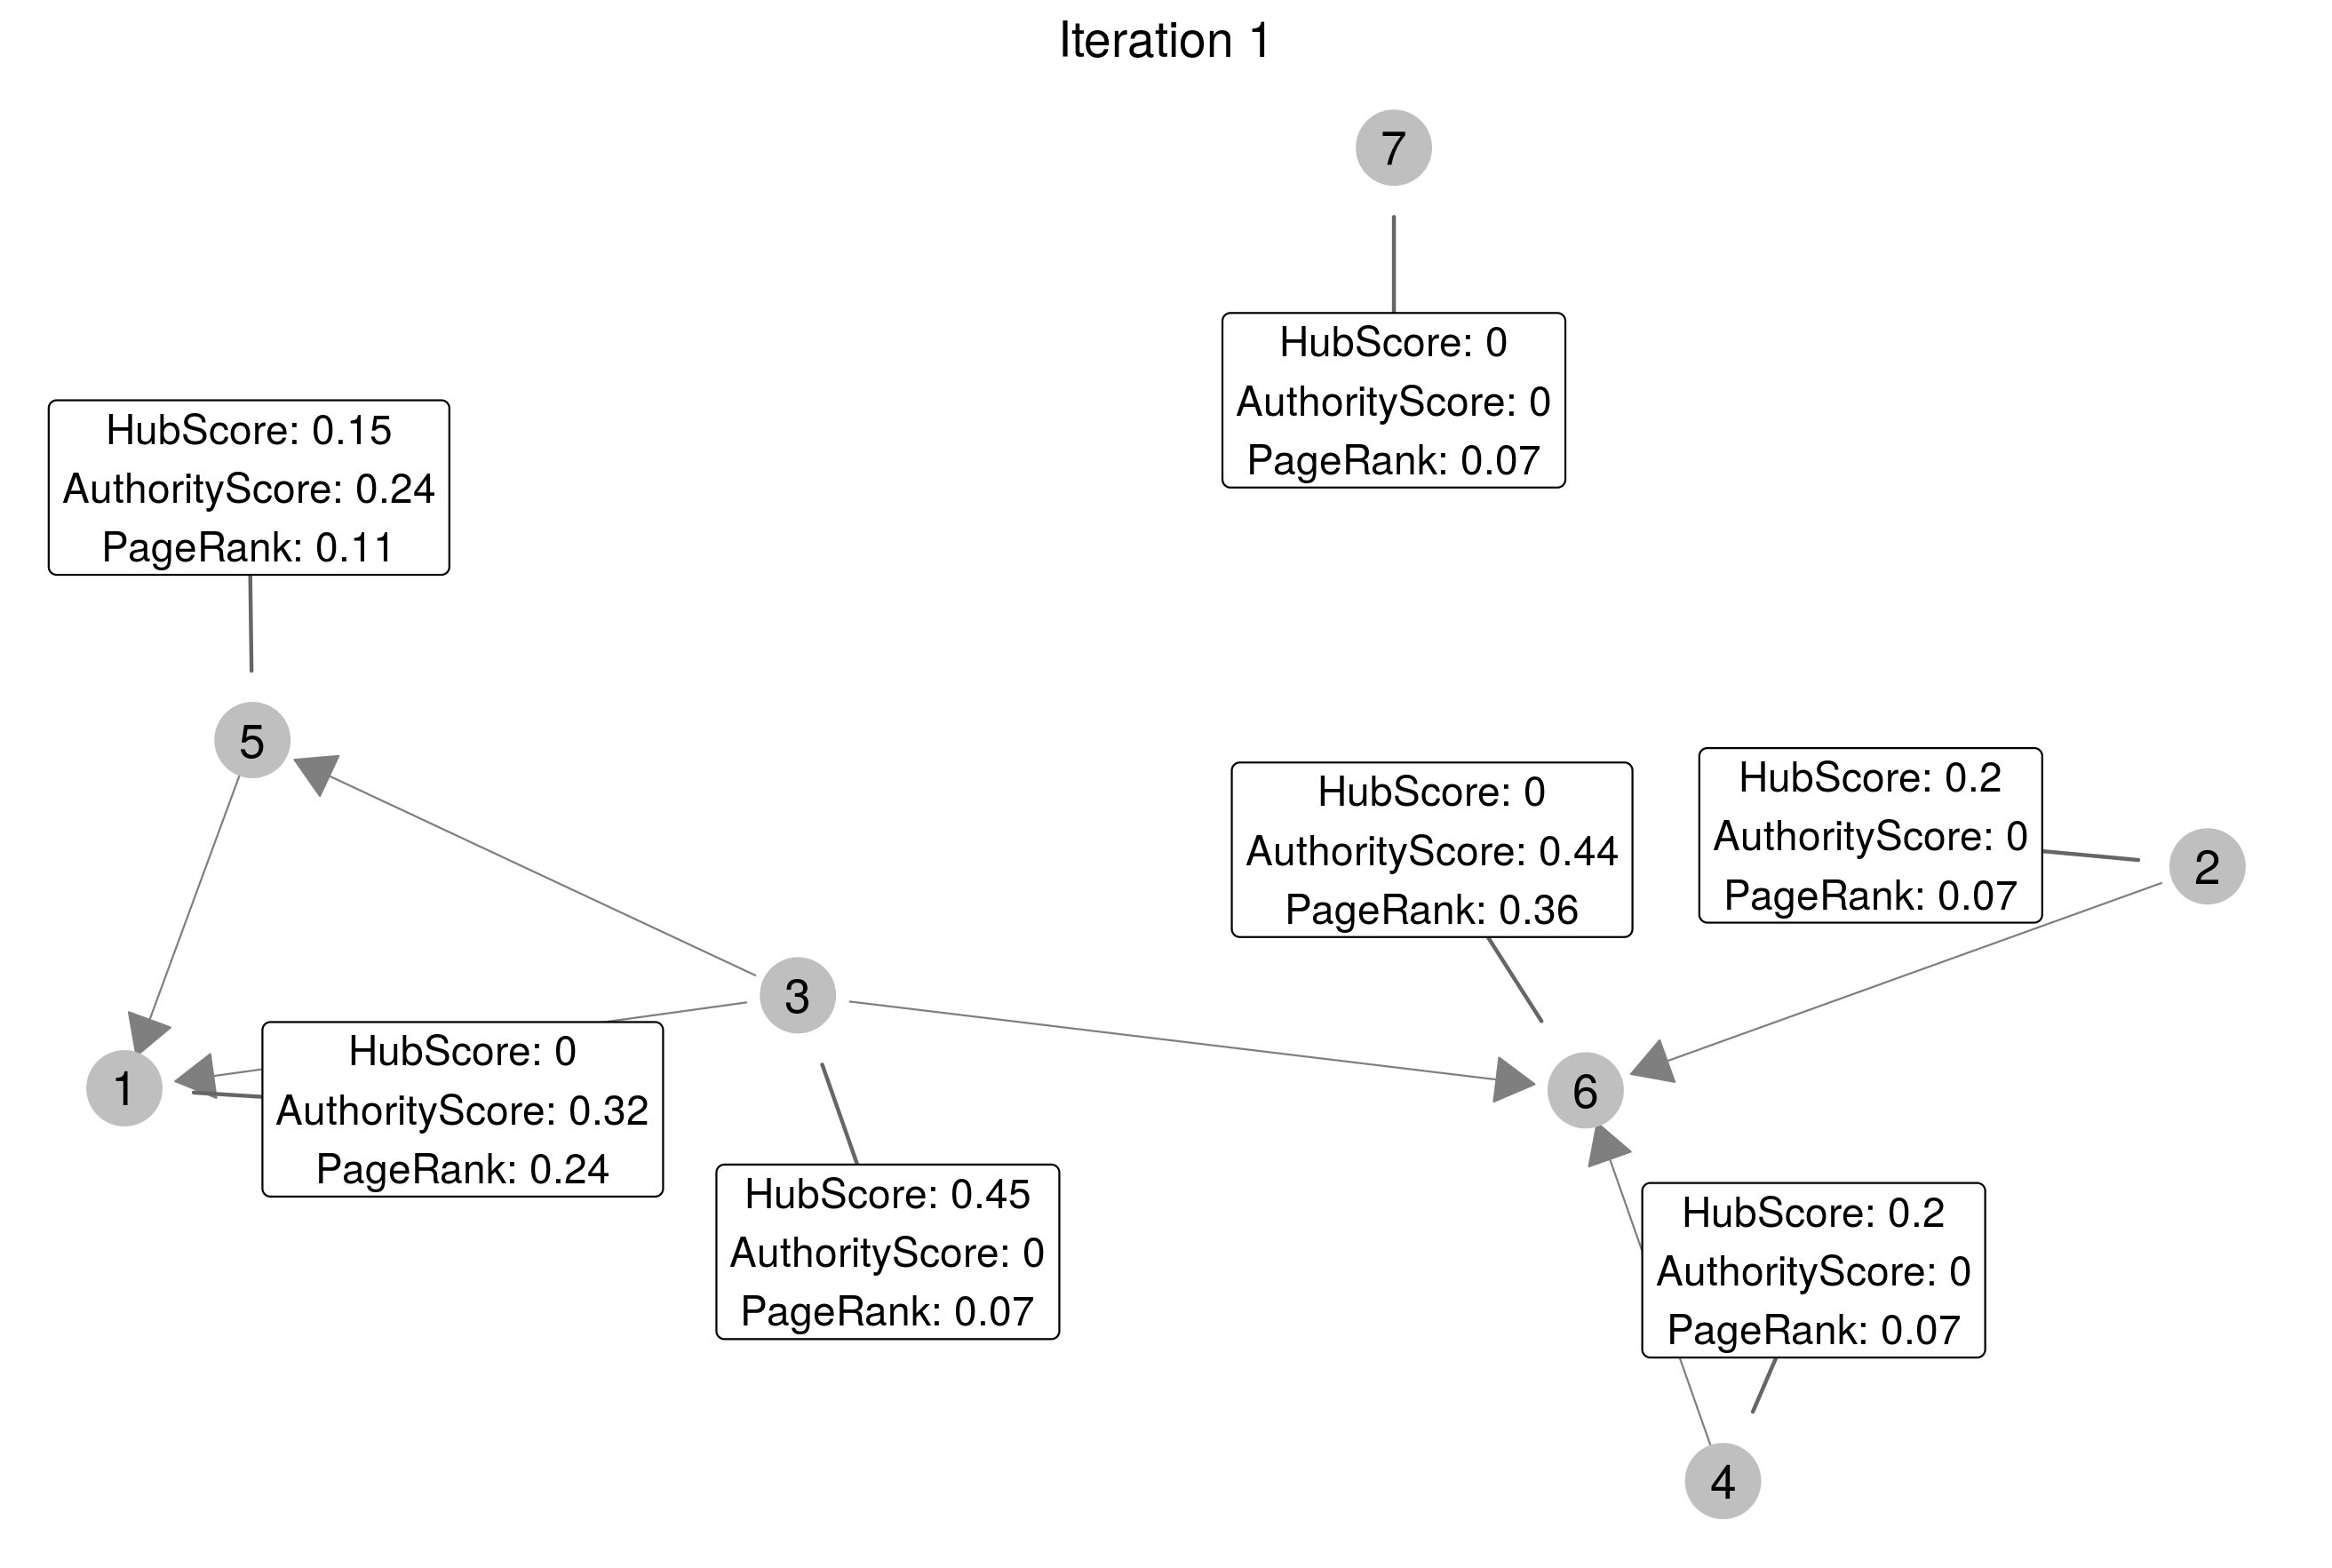
\includegraphics[scale=.8]{q1_iteration1.png}
\caption{Iteration 1}
\label{fig:q1_i1}
\end{figure}
\begin{figure}[H]
\centering
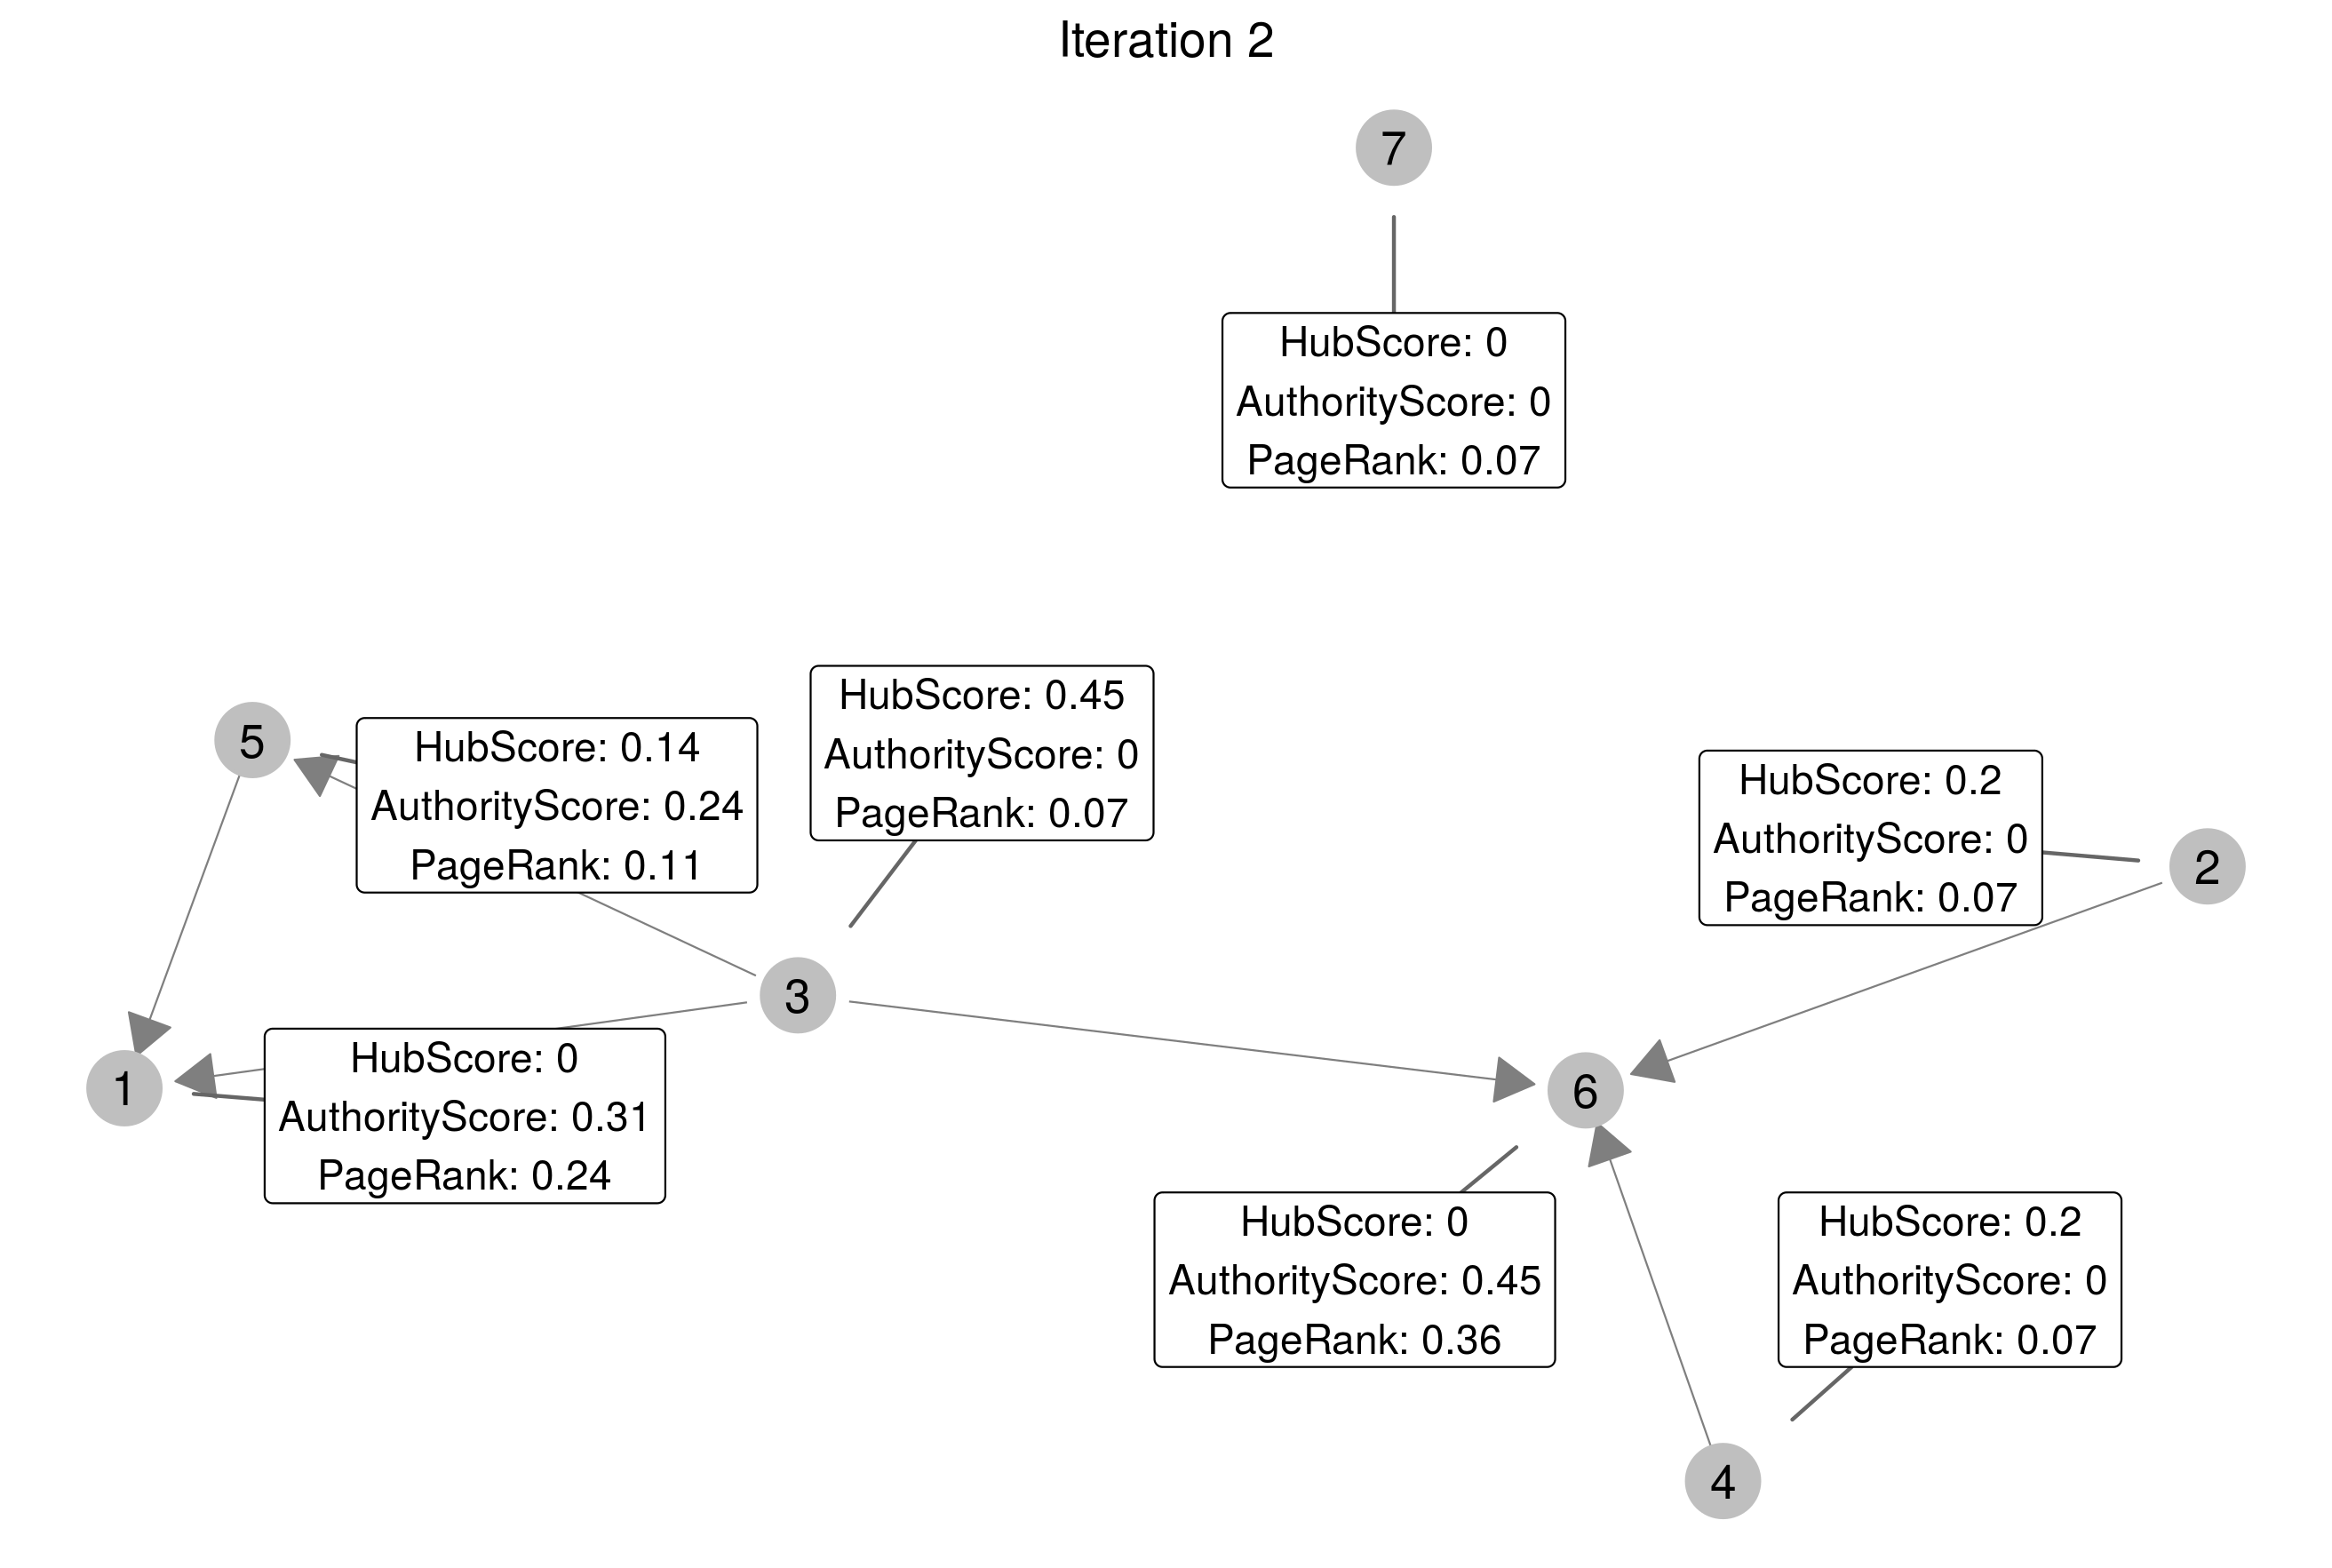
\includegraphics[scale=.8]{q1_iteration2.png}
\caption{Iteration 1}
\label{fig:q1_i2}
\end{figure}
\begin{figure}[H]
\centering
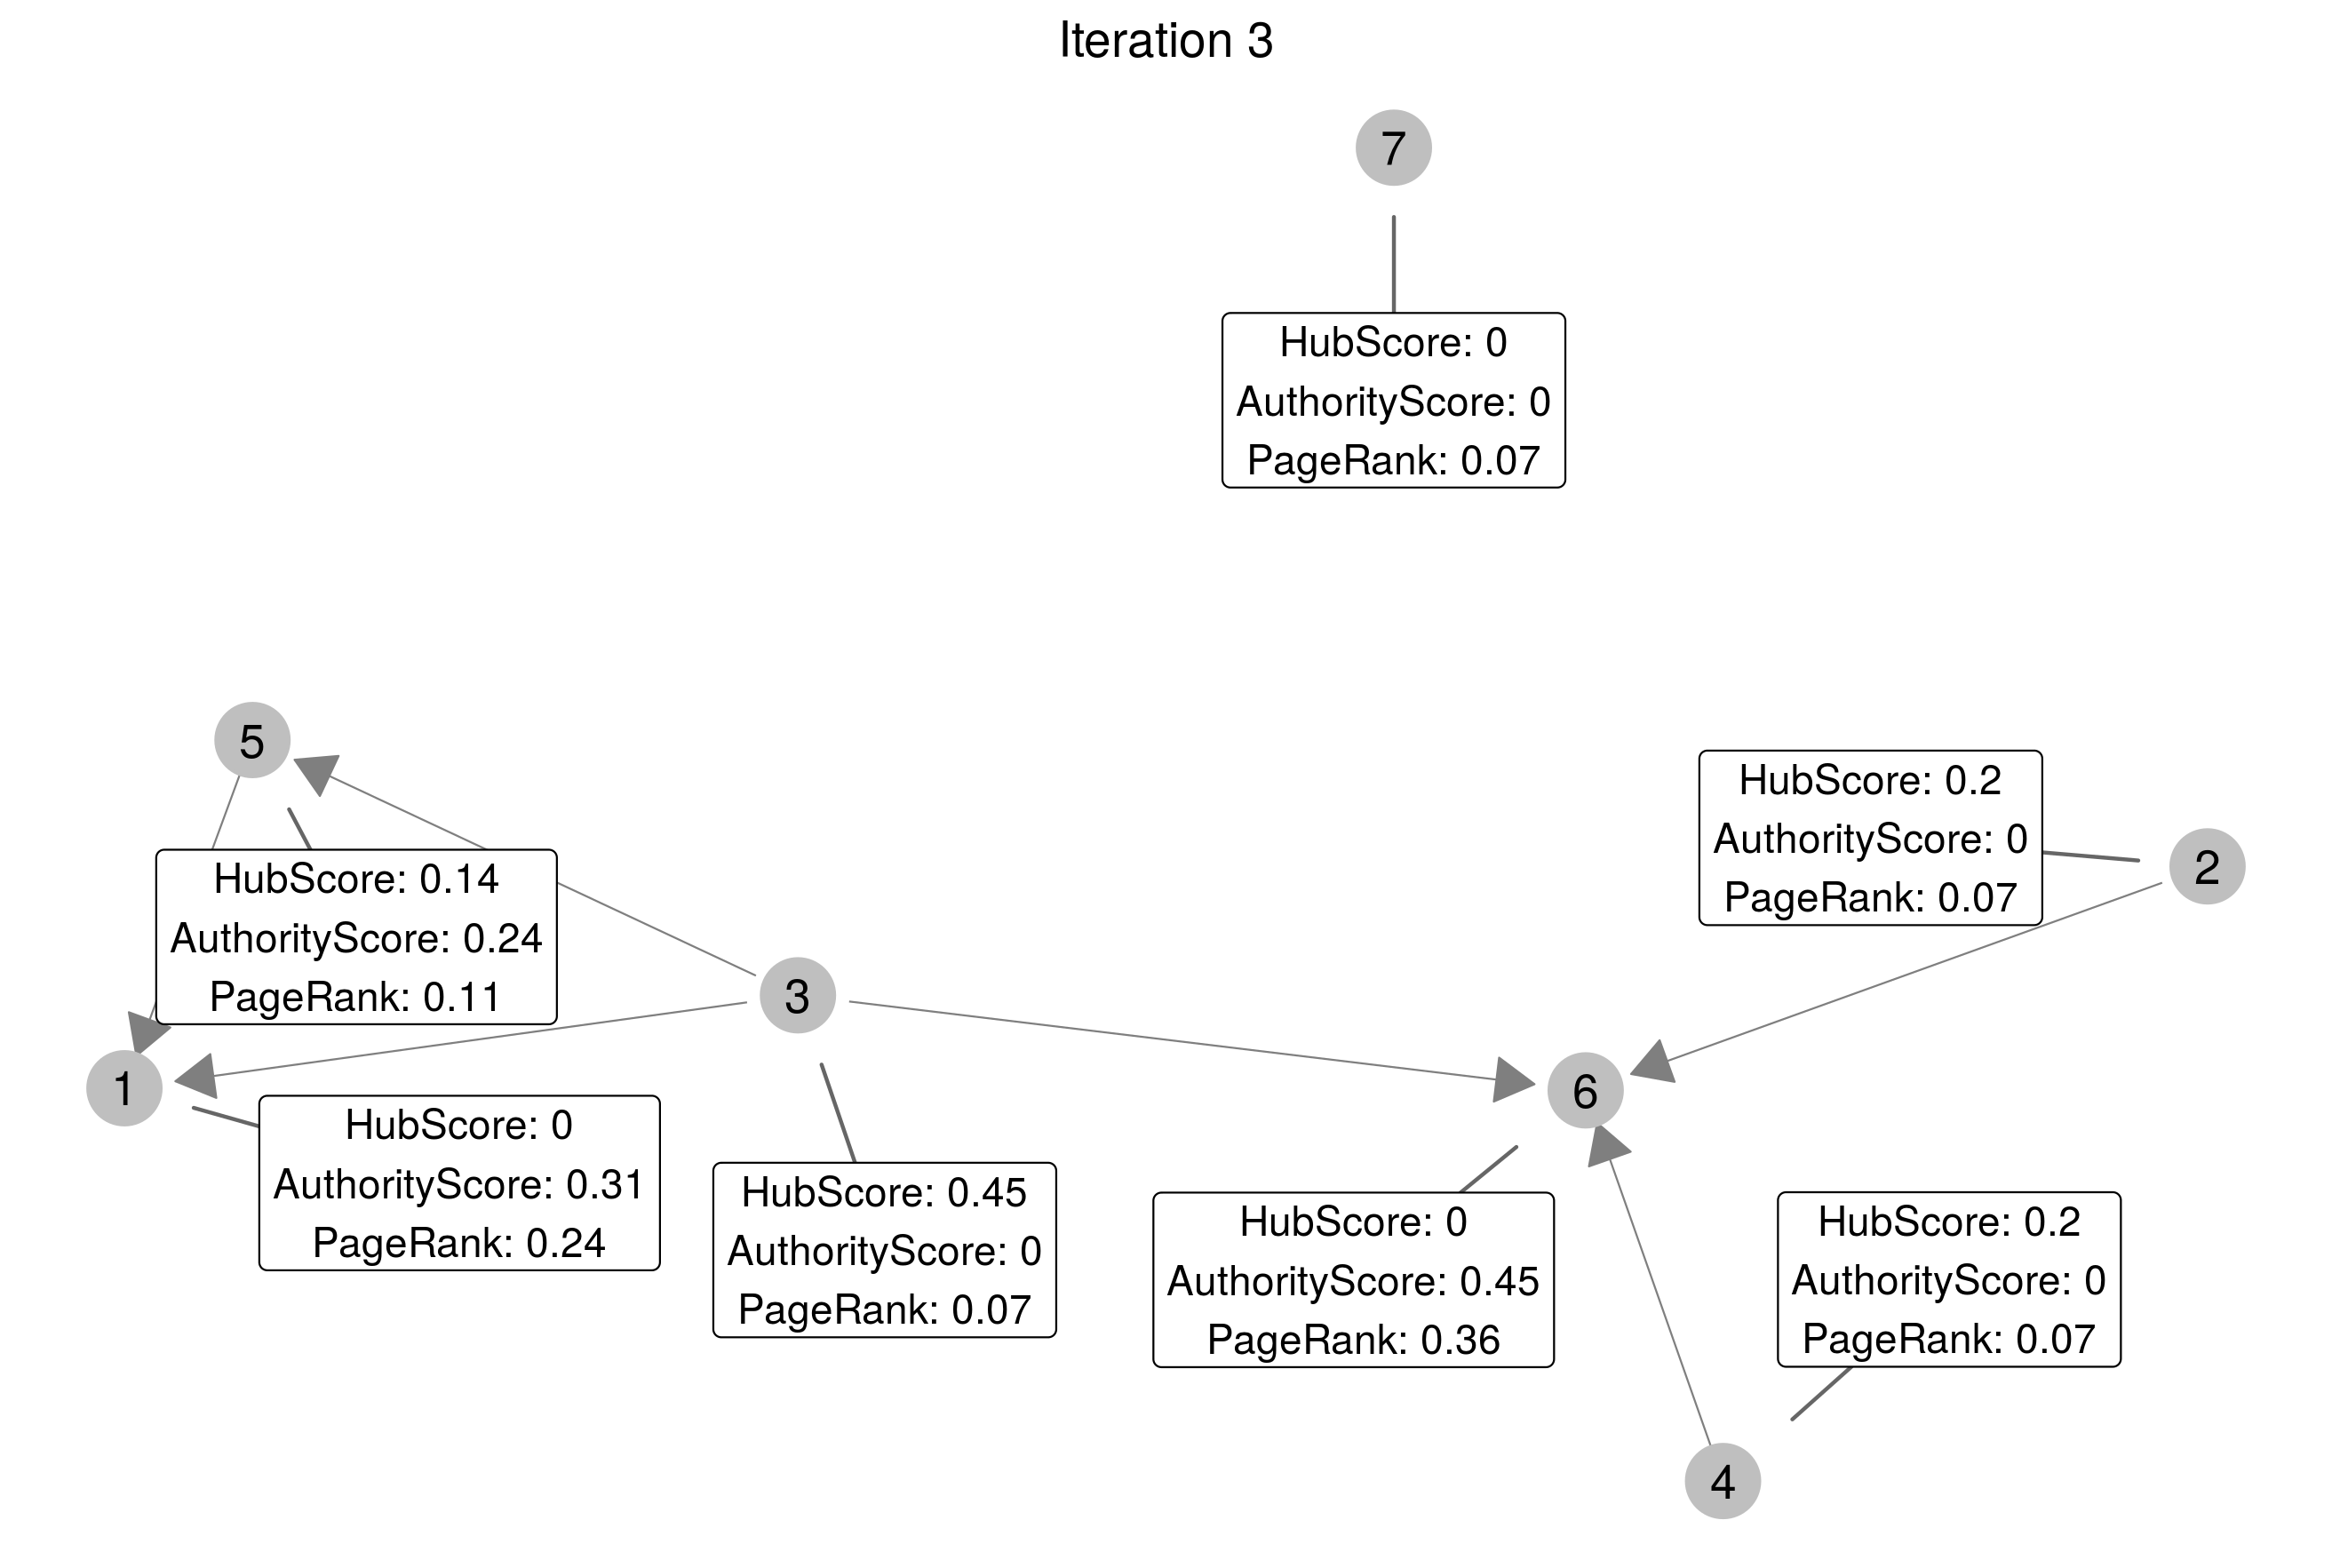
\includegraphics[scale=.8]{q1_iteration3.png}
\caption{Iteration 3}
\label{fig:q1_i3}
\end{figure}
\begin{figure}[H]
\centering
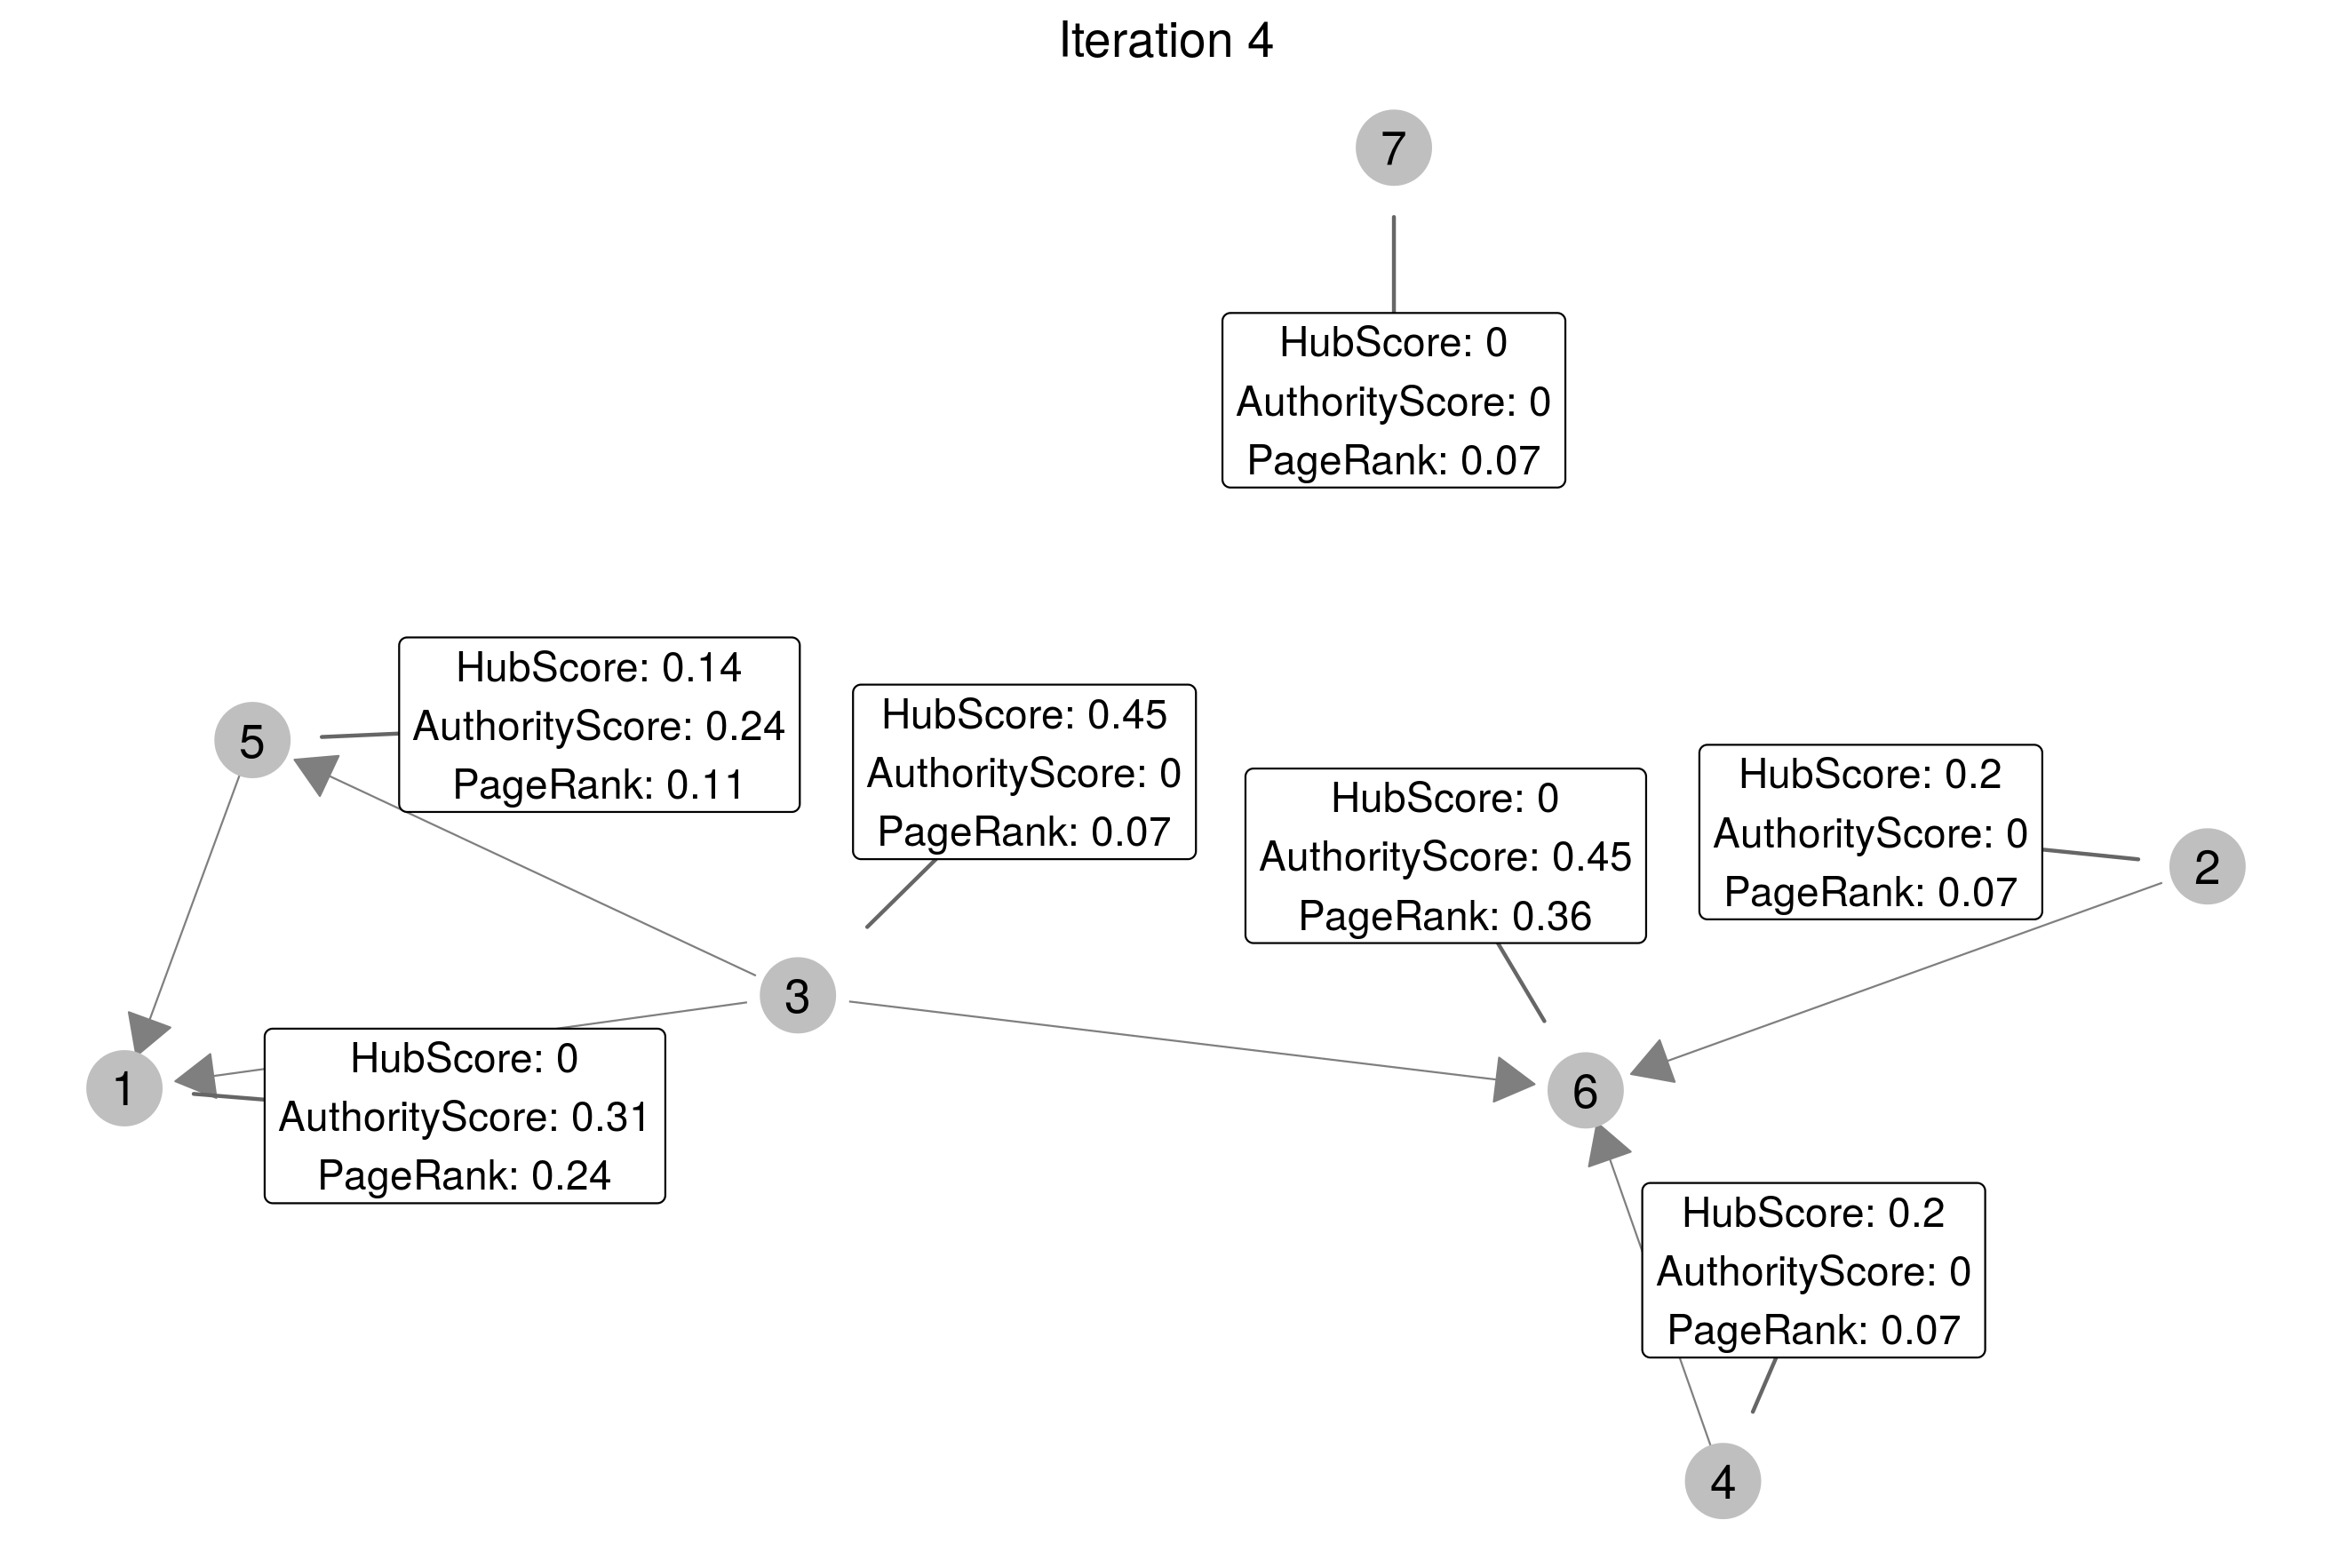
\includegraphics[scale=.8]{q1_iteration4.png}
\caption{Iteration 4}
\label{fig:q1_i4}
\end{figure}
\begin{figure}[H]
\centering
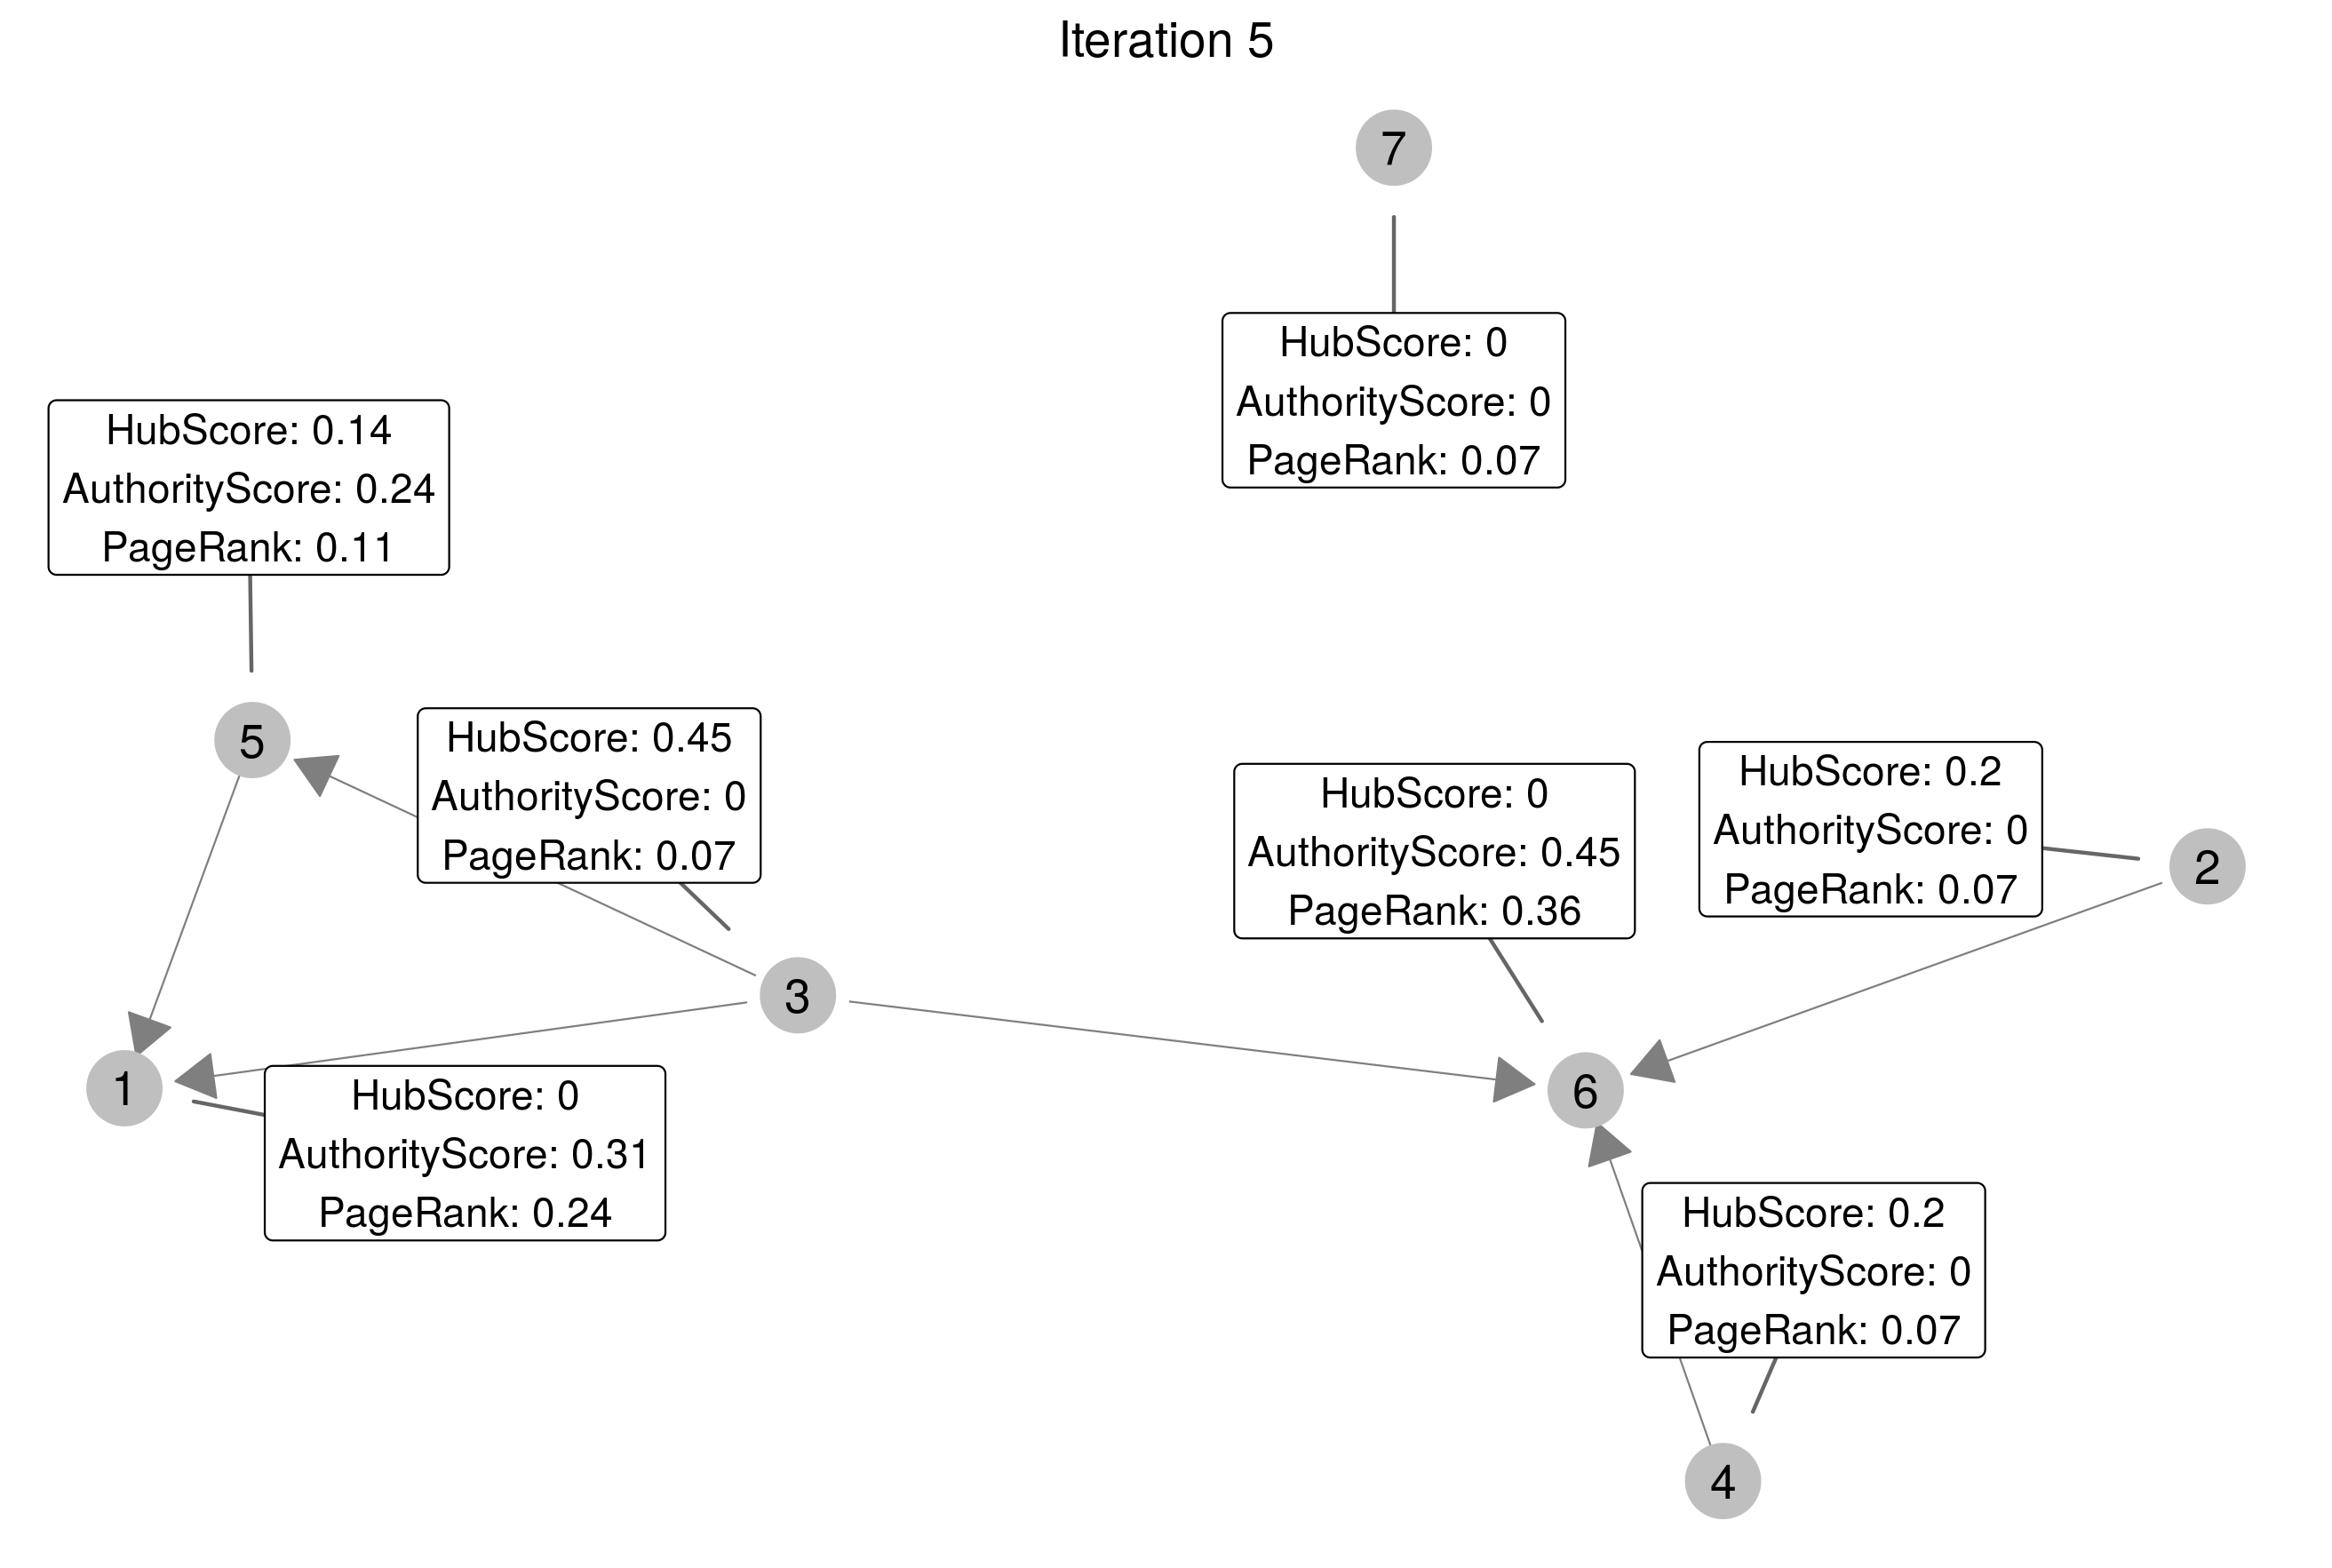
\includegraphics[scale=.8]{q1_iteration5.png}
\caption{Iteration 5}
\label{fig:q1_i5}
\end{figure}
\begin{code}
\captionof{listing}{Q1 Python} 
\label{code:q1p}
	\pycode{code/q1_10.3.py}
\end{code}
\begin{code}
\captionof{listing}{Q1 R} 
\label{code:q1r}
	\rcode{code/q1.R}
\end{code}
\newpage
\section{Question 10.6} \label{q2}
\begin{verbatim}
Find two examples of document filtering systems on the Web.  How do they build a profile for 
your information need?  Is the system static or adaptive?
\end{verbatim}
\subsection*{Answer} 
For my two examples I have choose Amazon and Spotify as both use an adaptive system for making recommendations to me.
\autoref{fig:q2_awhy} shows two snack food items I purchased together through Amazon both of which happen to be my all time favorite snack foods. 
\begin{figure}[H]
\centering
\adjustbox{trim={0} {3.1in} {0} {3cm},clip}%
{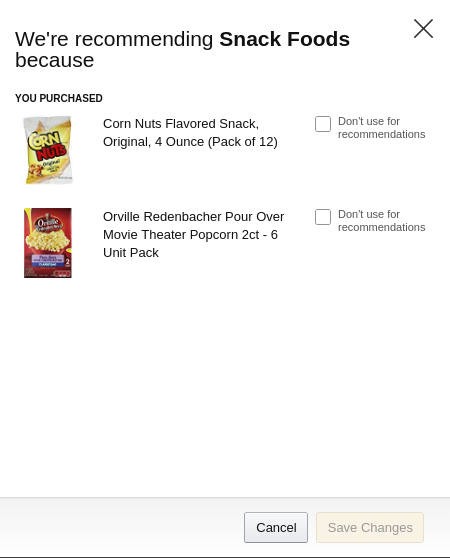
\includegraphics[scale=.8]{whyAmazonRecommened.png}}
\caption{Purchased Snack Foods}
\label{fig:q2_awhy}
\end{figure}
\noindent Ever since then I have been getting recommendations for similar snack foods as seen in \autoref{fig:q2_arec} which shows the first four recommendations. Both of the items I purchased had four and three fourth star ratings which was used in making the correlation to these recommended items \autoref{fig:q2_arec_ff}. Three of these recommendation are other Corn Nut products while the fourth is Jerky. This is included because other Amazon customers who bought Corn Nuts also purchased Jack Link's Beef Jerky with it \autoref{fig:q2_arec_bt}. This frequently bought item is also recommend for purchase with Corn Nuts when adding it to your cart.
\begin{figure}[H]
    \centering
    \begin{subfigure}[t]{0.5\textwidth}
        \centering
    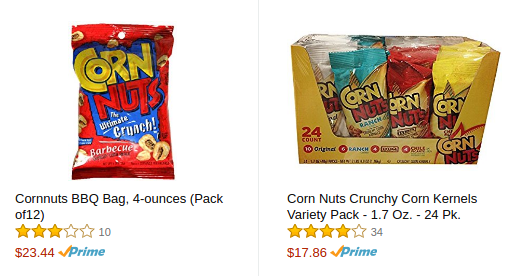
\includegraphics[scale=.6]{amazon_recp1.png}
     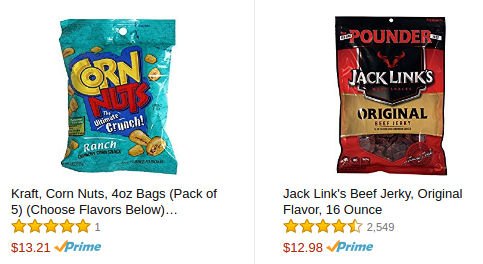
\includegraphics[scale=.6]{amazon_recp2.png}
          \caption{First Four Recommendations}
         \label{fig:q2_arec_ff}
    \end{subfigure}%
    ~ 
    \begin{subfigure}[t]{0.5\textwidth}
        \centering
      \adjustbox{trim={0} {1.2cm} {3in} {1.3cm},clip}%
{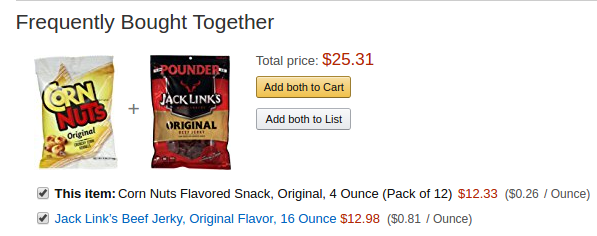
\includegraphics[scale=.7]{amazonCornFeq.png}}
        \caption{Frequently Bought With Corn Nuts}
          \label{fig:q2_arec_bt}
    \end{subfigure}
       \caption{Amazon Snack Food Recommendations}
    \label{fig:q2_arec}
\end{figure}
\noindent Amazon uses your purchase history and correlates it with purchases from other users who have also bought the same item as you to build its recommendations. My second example Spotify is an online music streaming service that allows for user created playlists, similar artists recommendations, top chart playlists and auto created playlists for a user.  \autoref{fig:q2_recpl} shows this weeks auto created playlist for me but most of the songs listed I am not familiar with by name. It was not until I listened to a few that I recognized them as they come from other user created playlists which I subscribe to. They were recommend to me because other users have \enquote{liked} the track i.e hit a check mark beside it after which it was saved to their like song list. Most of them were not too bad but the 4ware track by deadmau5 is excellent and one I liked as well after hearing it again via this recommended playlist.
\begin{figure}[H]
\centering
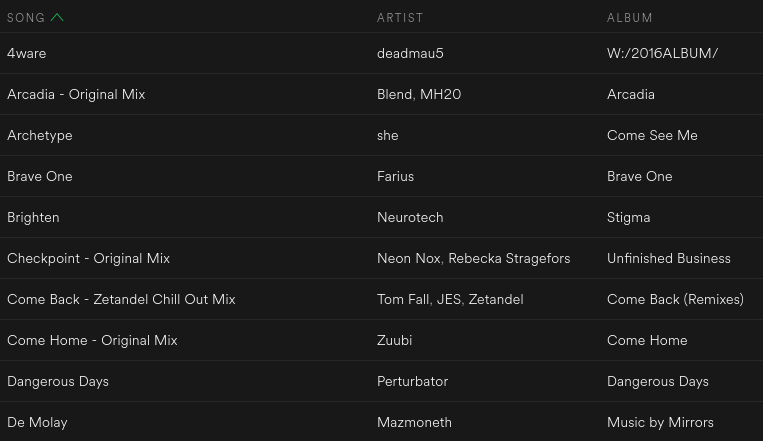
\includegraphics[scale=.6]{spotify_discover2.png}
   \caption{Recommended Playlist}
          \label{fig:q2_recpl}
\end{figure}
Since Spotify uses your listen history in combination with other users plus liked tracks to make recommendations and the recommendation is music the results can be weird at times or way off. For instance \autoref{fig:q2_snails} which shows the first three recommendations for similar albums based off listening to Nails. Nails is ultra aggressive hardcore/powerviolence band so the recommendations for Weekend Nachos and Cult Leader makes sense as they are in the sludgy cust punk powerviolence spectrums. Now Oathbreaker on the other hand is a post-hardcore band that has some tracks that could be called hardcore punk but that is up for debate. Looks like a bunch of wayward post-hardcorers like Nails and is why Spotify included in this recommendation.
\begin{figure}[H]
\centering
      \adjustbox{trim={0} {0} {2in} {0},clip}%
{
\includegraphics[scale=.5]{simToNails.png}}
   \caption{Suggestions Nails}
          \label{fig:q2_snails}
\end{figure}
\noindent As much as I would disagree with this recommendation it proves that Spotify is using an adaptive system to generate the recommendations it makes.
\clearpage
\section{Question 10.8} \label{q3}
\begin{verbatim}
Implement the nearest neighbor based collaborative filtering algorithm.
Using a publicly available collaborative filtering data set, compare the effective-
ness, in terms of mean squared error, of the Euclidean distance and correlation
similarity.
\end{verbatim}
\subsection*{Answer} 
I chose this question because it is a variation on assignment seven from cs532 Web Sciences and like that question I used the MoveLen dataset. 
But unlike that question I did not use the code submitted for it nor the code provided from the courses text book Programming Collective Intelligence. Instead I choose to use Pandas\footnote{\href{http://pandas.pydata.org/}{http://pandas.pydata.org/}} which is a high performance data analysis library akin to R. The source code used to generate the similarities can be seen in \autoref{code:q2cs} and \autoref{code:q2cs_help}.\newline 
\indent The MoveLen dataset contains 100,000 ratings (1-5) from 943 users for 1682 movies where each user has rated at least 20 movies. So computing the similarity for each user for a given k value would take some time as this user based similarity. In order to ensure the computation of k nearest neighbors  for an given k value for all users could be done relatively fast, the similarities for all users were computed, i.e 1 user vs 942 others 943 times. This was accomplished by processing 23 \enquote{\textit{chunks}} of 41 users 4 chunks at a time in parallel. Then for each user in a chunk the users similarity to every other user was computed using Euclidean distance and Pearson as the similarity measures. Once all chunks had been processed the results were combined into a single \ipy{pandas.DataFrame} and serialized to disk. This method of processing is much like the map and reduce paradigm. Instead of distributing the similarity computing function to multiple nodes pythons \ipy{multiprocess.Pool} applied that function to each chunk (map) using four different processes on my local machine and then combined (reduce) into a single result by the process which spawned them. \newline
\indent After the one vs all similarity for the users was computed the k nearest neighbors for $k=10$ was found for both similarity measures and \autoref{fig:q2_mse} show the mean squared error for both measures.
\begin{figure}[H]
\centering
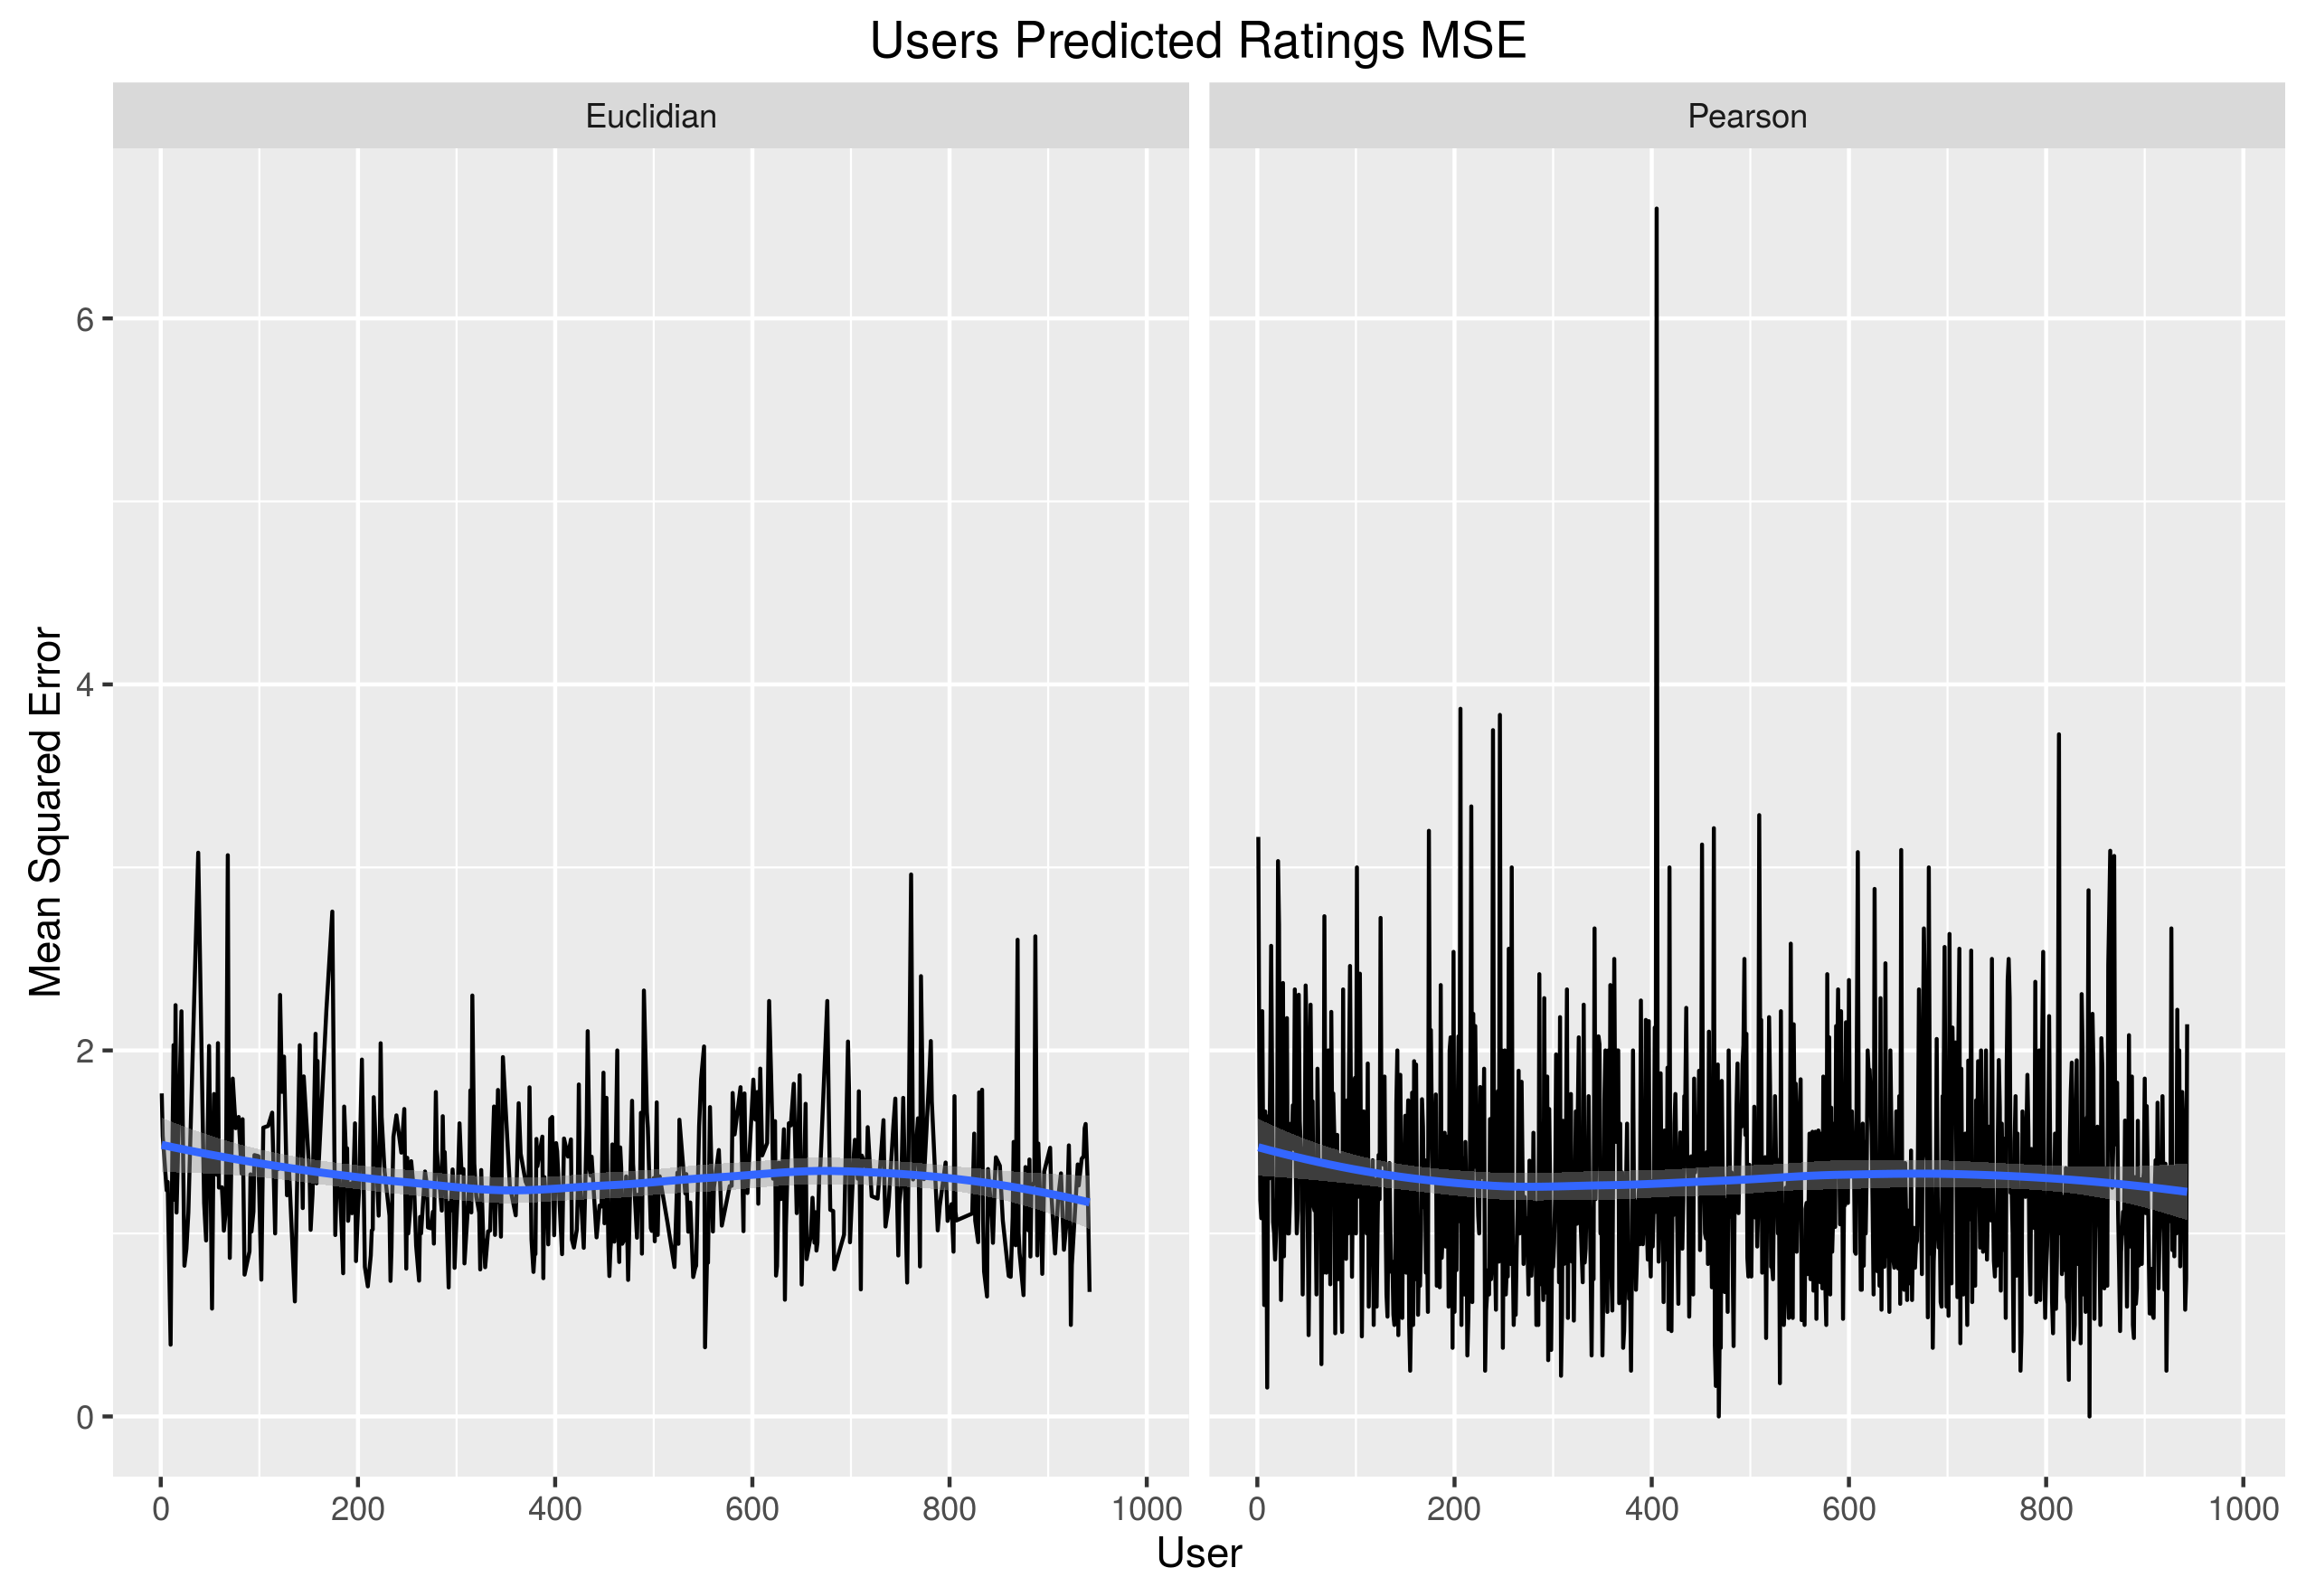
\includegraphics[scale=.8]{user_predicted_mse.png}
\caption{Predicted MSE}
\label{fig:q2_mse}
\end{figure}
\clearpage
Overall Euclidean distance measure performed the best whereas Pearsons had more extremes. The trend line for both measures shows they behave similarly even tho Pearson had higher MSE values overall. This is more easily seen when considering \autoref{fig:q2_p} and \autoref{fig:q2_u} which show a histogram (bin width = 50) of the ratings for both measures compared to the predicted values. Pearson, \autoref{fig:q2_p} predicted values that were $\rpm 1$ ranking than the actual. Euclidean distance faired similarly \autoref{fig:q2_u} but less so. The reason behind this could be attributed to the fact it is more suited to a clustering algorithm since it is more geared to this kind of problem than a true similarity function.
\begin{figure}[H]
\centering
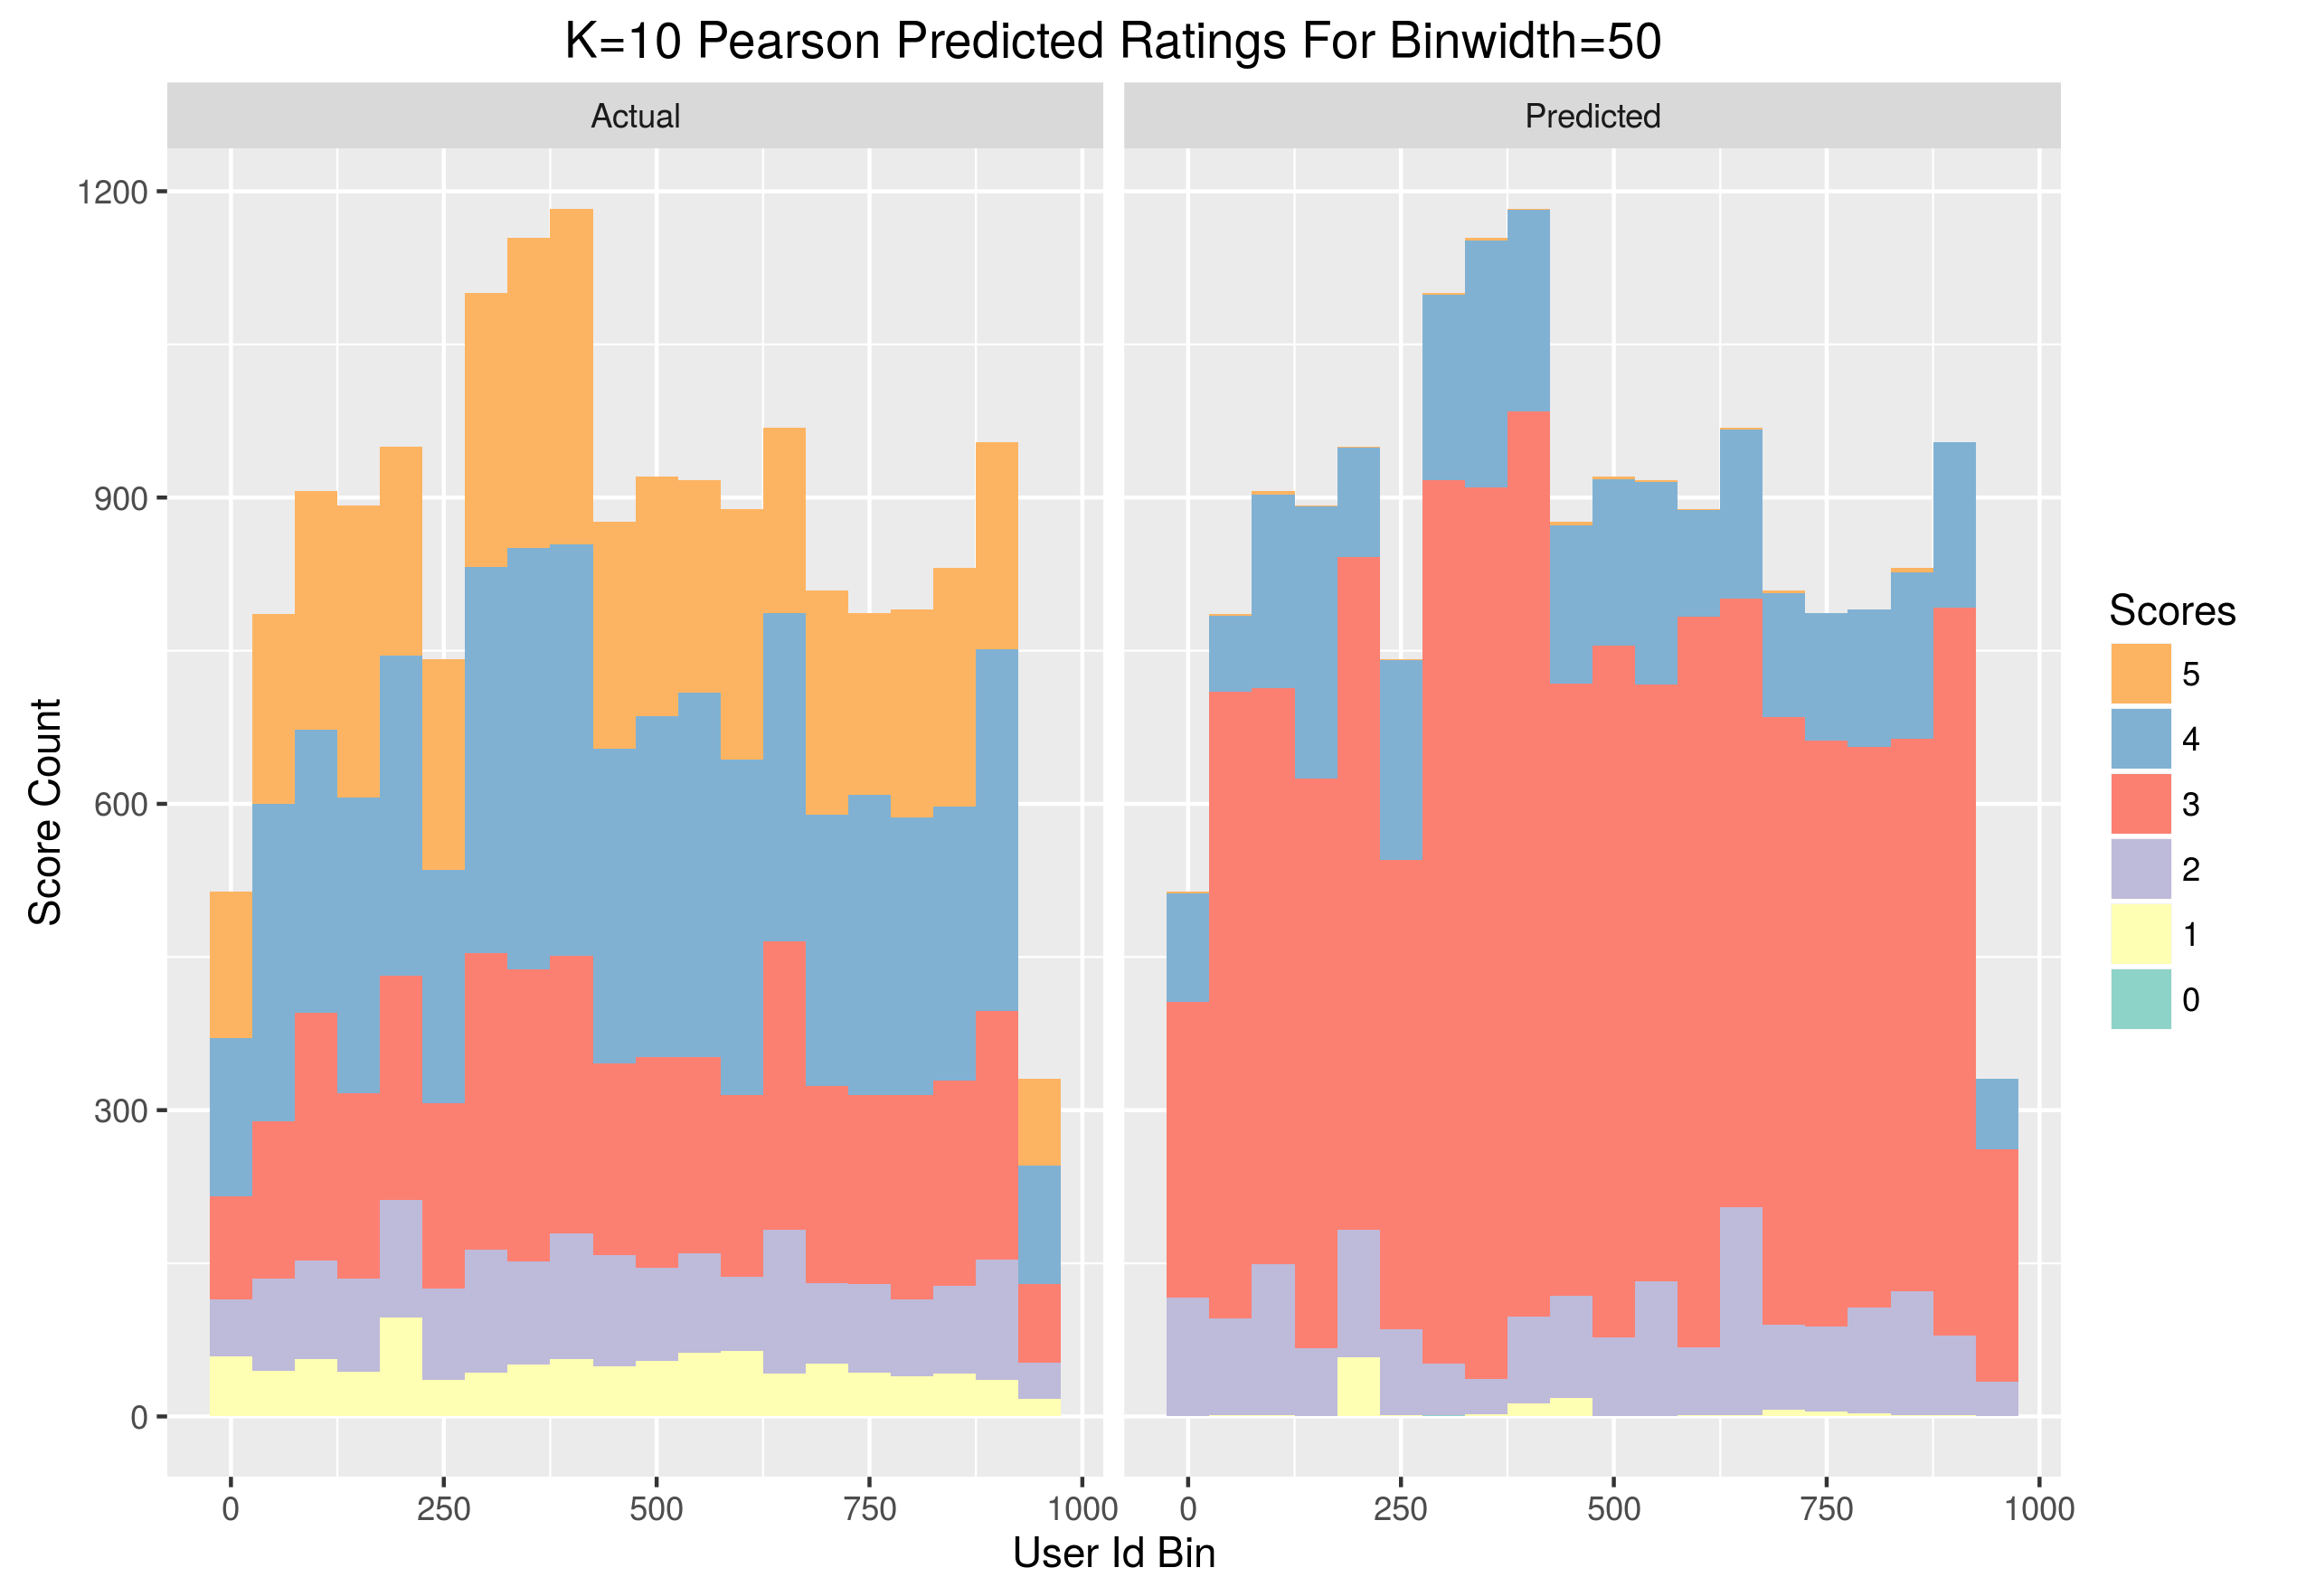
\includegraphics[scale=0.8]{pearson_predicted_buser.png}
\caption{User Prediction Pearson}
\label{fig:q2_p}
\end{figure}
\begin{figure}[H]
\centering
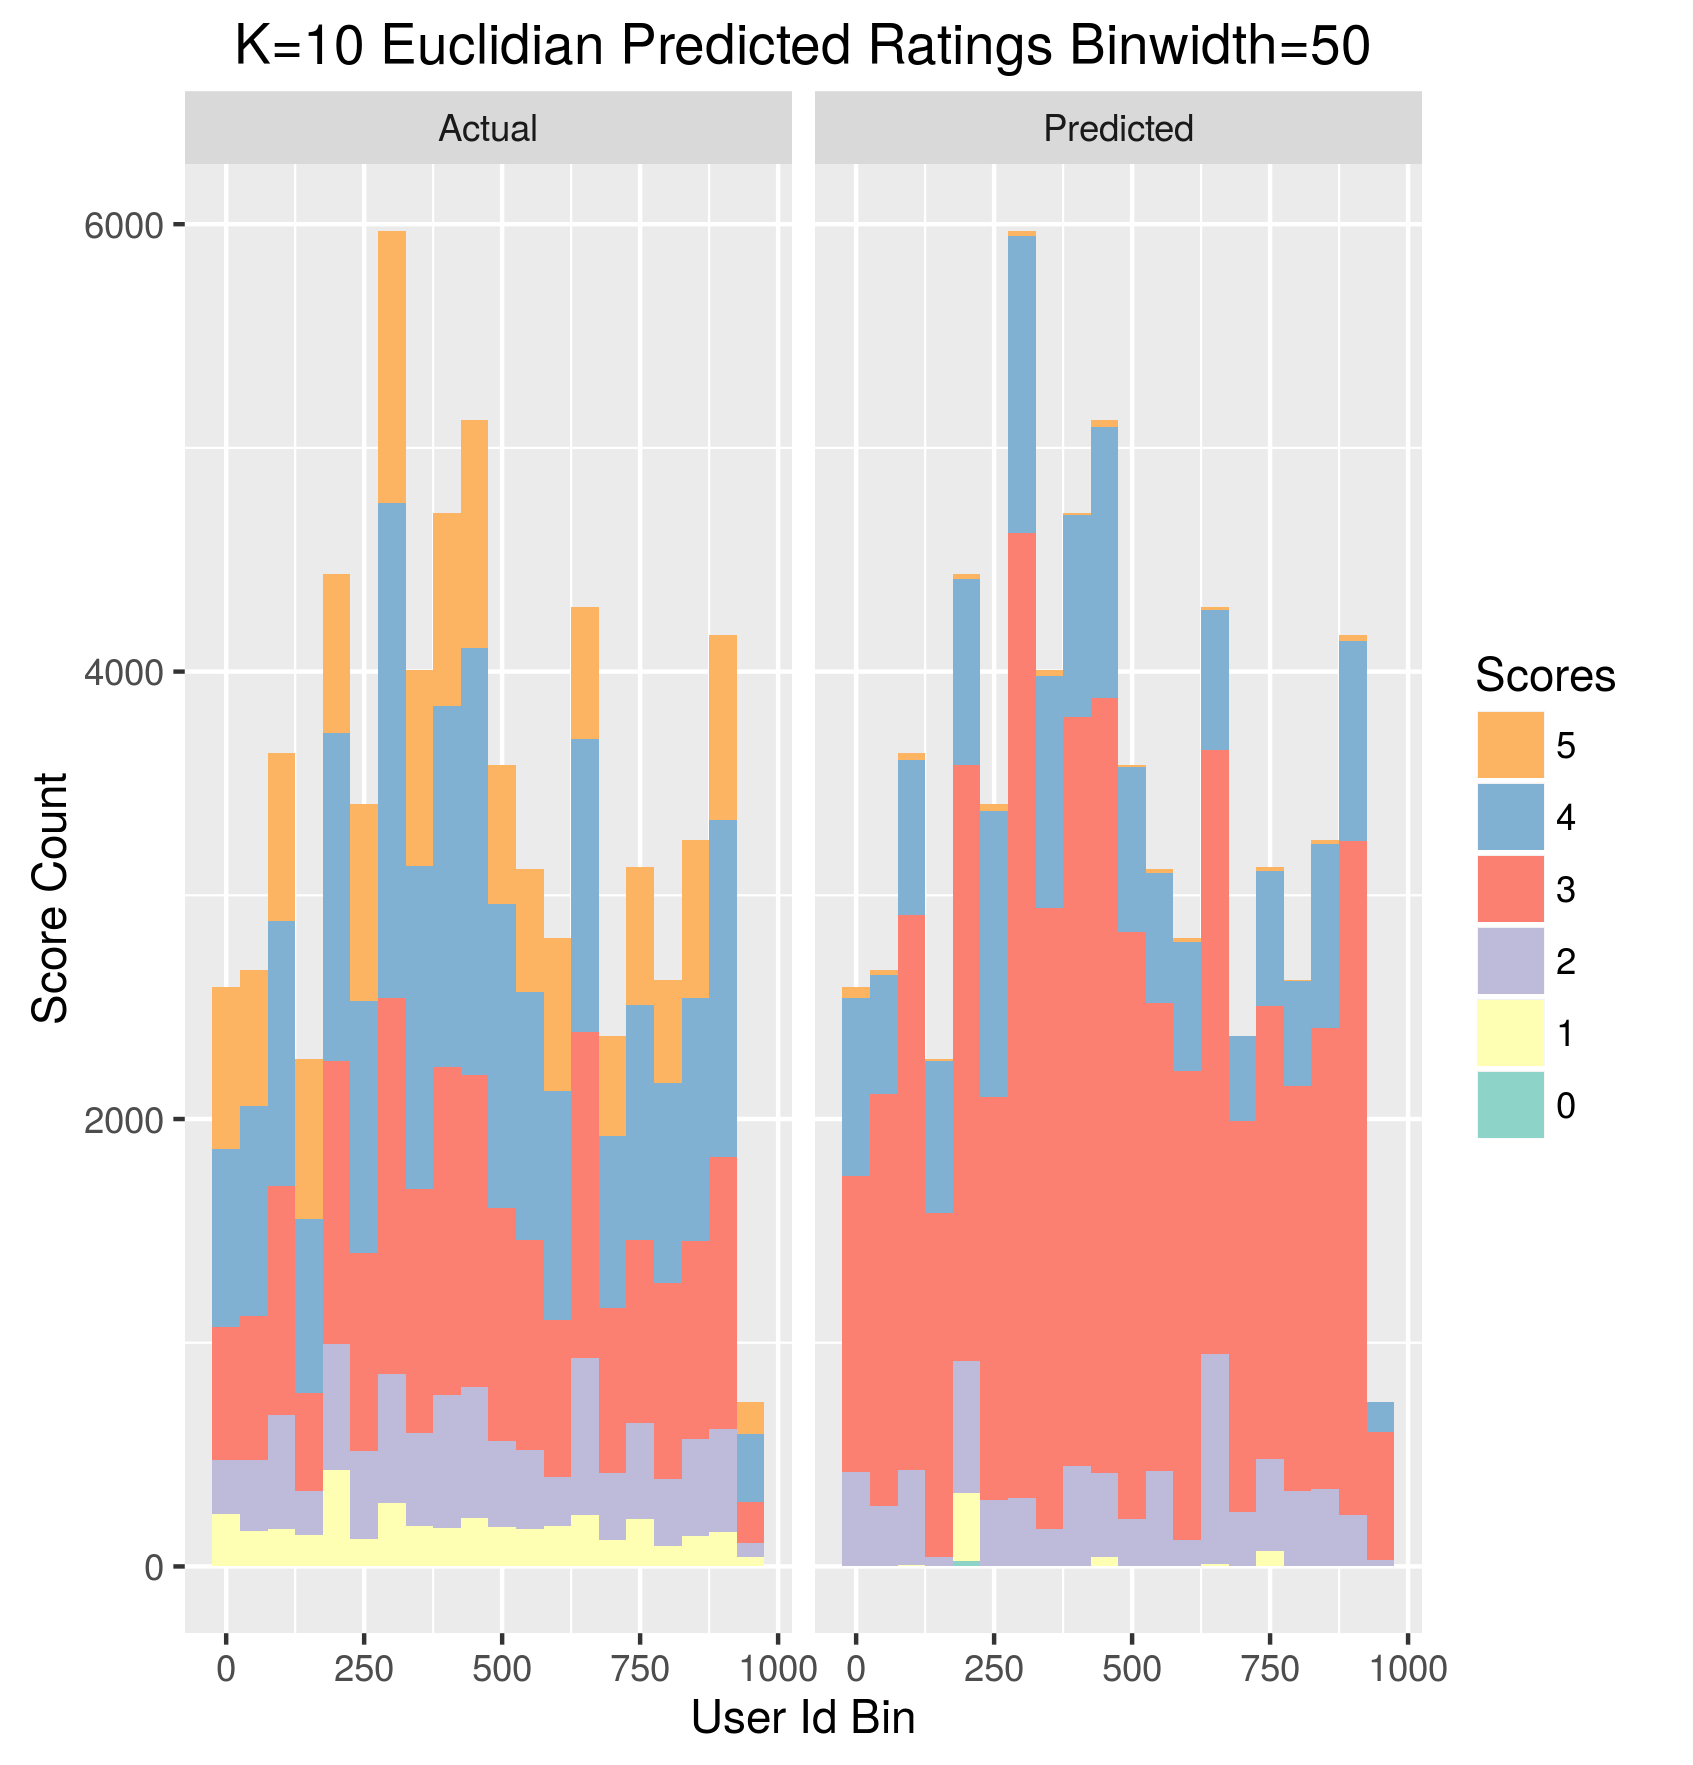
\includegraphics[scale=0.8]{euclid_predicted_buser.png}
\caption{User Prediction Euclidean Distance}
\label{fig:q2_u}
\end{figure}

\begin{code}
\captionof{listing}{Q2 Compute Similarities} 
\label{code:q2cs}
	\pycode{code/q2_10.8.py}
\end{code}
\begin{code}
\captionof{listing}{Q2 Generate Graphs} 
\label{code:q2rgg}
	\rcode{code/q2_plotter.R}
\end{code}
\begin{code}
\captionof{listing}{Q2 Compute Similarities Helper} 
\label{code:q2cs_help}
	\pycode{code/q2_helpers.py}
\end{code}
\begin{code}
\captionof{listing}{Q2 Generate Graphs Helper} 
\label{code:q2rgg_help}
	\rcode{code/q2_plotter_helper.R}
\end{code}
\clearpage
\section{Question 11.2} \label{q4}
\begin{verbatim}
Does your favorite web search engine use a bag of words representation?
How can you tell whether it does or doesn’t?
\end{verbatim}
\subsection*{Answer} 
Unlike the vast majority of the world my favorite search engine is \href{https://duckduckgo.com}{duckduckgo.com} because that's so met\anarchy{}l but in all seriousness I like it because it is a \href{https://duckduckgo.com/about}{privacy} first search engine.
\newpage
\section{Extra Credit Wiki Small} \label{q5}
\begin{verbatim}
Turn in with A5, 8 points available. Download the wikipedia.org URIs from the live web.

summarize the HTTP status codes returned,all 200? Redirections? 404s? 
do we still have 6043 documents? or have their been splits & merges 
 (see also: wikipedia disambiguation pages)? (1 pt)

compare and contrast the in- and out-links from this collection. the number, 
the domains linked to, the HTTP status of the non-wikipedia links in the article 
(i.e., are they 200, 404, or something else?). (1 pt)

Compare the least and most popular articles (in terms of in-links) in the 2008 snapshot 
vs. the least and most popular articles in your 2015 snapshot. (1 pt)

compare and contrast the anchor text for the articles in the collection: 
are we gaining or losing terms? (1 pt)

compare and contrast the sizes of the same pages (i.e., 2008 vs. 2015) in: (2 pts)
• bytes
• total terms
• total unique terms

for all of the pages (i.e., treat each collection as a single unit), 
compare the 2008 vs. 2015 snapshots in: (2pts)
• bytes
• total terms
• total unique terms
\end{verbatim}
\subsection{Answer} 
\newpage
\begin{code}
\captionof{listing}{General Utility Functions} 
\label{code:util}
	\pycode{code/util.py}
\end{code}
\begin{code}
\captionof{listing}{Modified NX Hits and Pagerank Algos} 
\label{code:nxc}
	\pycode{code/nx_controled_algos.py}
\end{code}
\begin{code}
\captionof{listing}{Updated Context Classes} 
\label{code:cntxc}
	\pycode{code/contextClasses.py}
\end{code}
\end{document}